\documentclass[journal]{style/vgtc} 			          % final (journal style)
%\documentclass[review,journal]{style/vgtc}         % review (journal style)
%\documentclass[widereview]{style/vgtc}             % wide-spaced review
%\documentclass[preprint,journal]{style/vgtc}       % preprint (journal style)
%\documentclass[electronic,journal]{style/vgtc}     % electronic version, journal
%% Uncomment one of the lines above depending on where your paper is
%% in the conference process. ``review'' and ``widereview'' are for review
%% submission, ``preprint'' is for pre-publication, and the final version
%% doesn't use a specific qualifier. Further, ``electronic'' includes
%% hyperreferences for more convenient online viewing.
%% Please use one of the ``review'' options in combination with the
%% assigned online id (see below) ONLY if your paper uses a double blind
%% review process. Some conferences, like IEEE Vis and InfoVis, have NOT
%% in the past.

%% Please note that the use of figures other than the optional teaser is not permitted on the first page
%% of the journal version.  Figures should begin on the second page and be
%% in CMYK or Grey scale format, otherwise, colour shifting may occur
%% during the printing process.  Papers submitted with figures other than the optional teaser on the
%% first page will be refused.

%% These three lines bring in essential packages: ``mathptmx'' for Type 1
%% typefaces, ``graphicx'' for inclusion of EPS figures. and ``times''
%% for proper handling of the times font family.

\usepackage{mathptmx}
\usepackage{graphicx}
\usepackage{times}

% -- My Own Packages and Commands
\usepackage[normalem]{ulem}
\usepackage{xcolor}
\newcommand{\rem}[1]{\textcolor{red}{\sout{#1}}}
\newcommand{\add}[1]{\textcolor{blue}{\uline{#1}}}
\newcommand{\com}[1]{\textcolor{orange}{\uline{#1}}}

%% We encourage the use of mathptmx for consistent usage of times font
%% throughout the proceedings. However, if you encounter conflicts
%% with other math-related packages, you may want to disable it.

%% This turns references into clickable hyperlinks.
\usepackage[bookmarks,backref=true,linkcolor=black]{hyperref} %,colorlinks
\hypersetup{
  pdfauthor = {},
  pdftitle = {},
  pdfsubject = {},
  pdfkeywords = {},
  colorlinks=true,
  linkcolor= black,
  citecolor= black,
  pageanchor=true,
  urlcolor = black,
  plainpages = false,
  linktocpage
}

%% If you are submitting a paper to a conference for review with a double
%% blind reviewing process, please replace the value ``0'' below with your
%% OnlineID. Otherwise, you may safely leave it at ``0''.
%% TODO: Blind Review: Replace with online ID
\onlineid{175}

%% declare the category of your paper, only shown in review mode
\vgtccategory{Research}

%% allow for this line if you want the electronic option to work properly
\vgtcinsertpkg

%% In preprint mode you may define your own headline.
%\preprinttext{To appear in an IEEE VGTC sponsored conference.}

%% Paper title.
%% TODO: Replace towards with regarding?

\title{Regression Cube Analysis of Cohort Study Data}

%% This is how authors are specified in the journal style

%% indicate IEEE Member or Student Member in form indicated below
\author{Paul Klemm, Kai Lawonn, Sylvia Gla{\ss}er, Uli Niemann, Katrin Hegenscheid, Henry V{\"o}lzke, Bernard Preim}
\authorfooter{
%% insert punctuation at end of each item
\item
 Paul Klemm, Kai Lawonn, Sylvia Gla{\ss}er, Uli Niemann, Bernhard Preim are with Otto-von-Guericke University Magdeburg, Germany. E-mail: \{klemm,lawonn,glasser,niemann,preim\}@ovgu.de
\item
 Katrin Hegenscheid, Henry V{\"o}lzke are with Ernst-Moritz-Arndt University Greifswald, Germany. E-mail: \{katrin.hegenscheid,voelzke\}@uni-greifswald.de
}

%other entries to be set up for journal
\shortauthortitle{Klemm \MakeLowercase{\textit{et al.}}: Regression Cube Analysis of Cohort Study Data}
%\shortauthortitle{Firstauthor \MakeLowercase{\textit{et al.}}: Paper Title}

%% Abstract section.
\abstract{%
%\com{Problem}.
Epidemiological studies comprise heterogeneous data about a subject group (a \emph{cohort}) to define disease-specific risk factors.
%%
These data contain information (\emph{features}) about a subject's lifestyle, medical condition as well as medical image data.
%%
%These features are analyzed using statistical regression analysis to identify feature combinations indicating a disease (the \emph{target feature}).
%%
Statistical regression analysis is used to evaluate these features and to identify feature combinations indicating a disease (the \emph{target feature}).
%%
Although there is a strong demand for overview visualizations of a whole data set towards a target feature, no suitable tool is available for epidemiological researchers.

%\com{New Solution}.
%%
We propose an analysis approach of epidemiological data sets by incorporating all features in an exhaustive regression-based analysis.
%%
This approach combines all \emph{independent features} with respect to a \emph{target feature} and provides a visualization, which reveals insights into the data by highlighting relationships.
%%
A 3D-visualization of all combinations of two to three independent features towards a target acts as an overview of the whole data set, the \emph{Regression Cube}.
%%
Slicing through the \emph{Regression Cube} allows for the detailed analysis of features towards the target disease.
%%
Expert knowledge about disease-specific hypotheses can be included into the analysis by adjusting the regression model formulas.
%%
Furthermore, the influences of features can be assessed using a difference view comparing different calculation results.
%%
%\com{Validation \& Results}.
%%
We applied our \emph{Regression Cube} method to a hepatic steatosis data set to reproduce results from a data-mining driven analysis.
%%
A qualitative analysis with three domain experts was conducted on a breast fat data set.
%%
We were able to derive new hypotheses about relations between breast fat density and breast lesions towards breast cancer.
%%
%\com{Implications}.
%%
%With our work, we present a visual overview of epidemiological data with the \emph{Regression Cube}, which allows for the first time an interactive regression-based analysis of large feature sets with respect to a disease.
} % end of abstract

%% Keywords that describe your work. Will show as 'Index Terms' in journal
%% please capitalize first letter and insert punctuation after last keyword
\keywords{Interactive Visual Analysis, Epidemiology, Breast Cancer, Hepatic Steatosis}

%% ACM Computing Classification System (CCS). 
%% See <http://www.acm.org/class/1998/> for details.
%% The ``\CCScat'' command takes four arguments.

\CCScatlist{ % not used in journal version
 \CCScat{K.6.1}{Management of Computing and Information Systems}%
{Project and People Management}{Life Cycle};
 \CCScat{K.7.m}{The Computing Profession}{Miscellaneous}{Ethics}
}

%% Uncomment below to include a teaser figure.
  % \teaser{
  % \centering
  % \includegraphics[width=16cm]{CypressView}
  % \caption{In the Clouds: Vancouver from Cypress Mountain.}
  % }

%% Uncomment below to disable the manuscript note
%\renewcommand{\manuscriptnotetxt}{}

%% Copyright space is enabled by default as required by guidelines.
%% It is disabled by the 'review' option or via the following command:
% \nocopyrightspace

%%%%%%%%%%%%%%%%%%%%%%%%%%%%%%%%%%%%%%%%%%%%%%%%%%%%%%%%%%%%%%%%
%%%%%%%%%%%%%%%%%%%%%% START OF THE PAPER %%%%%%%%%%%%%%%%%%%%%%
%%%%%%%%%%%%%%%%%%%%%%%%%%%%%%%%%%%%%%%%%%%%%%%%%%%%%%%%%%%%%%%%

\begin{document}

%% The ``\maketitle'' command must be the first command after the
%% ``begin{document}'' command. It prepares and prints the title block.

%% the only exception to this rule is the \firstsection command
\firstsection{Introduction}

\maketitle
%%
Epidemiology aims to characterize health and disease conditions in defined populations (\emph{cohorts}).
%%
Insights about risk factors allow to characterize disease-specific high-risk groups and act as important diagnostic key figures \cite{Fletcher2012}.
%%
Furthermore, they can be used to derive recommendations regarding a healthy lifestyle or to provide information about wide-spread diseases.
%%
During the standard workflow, physicians transform observations into hypotheses, which are depicted using epidemiological features and then assessed using regression analyses.

An important epidemiological tool for deriving such features is the evaluation of a \emph{cohort study}, such as the Study of Health in Pomerania (SHIP) \cite{Volzke2011}.
%%
To reduce any selection bias, subjects are randomly invited without a focus on a specific disease.
%%
Hence, a wide range of features is acquired.
%
Social and lifestyle factors, prior or current diseases and medications as well as medical parameters, such as blood pressure, are gathered.
%%
Medical image data from non-radiating modalities, e.g., magnetic resonance imaging (MRI), is also acquired in modern studies.
%%
These data may be quantified based on user-defined landmarks, which describe attributes like the shape, the volume or the diameter of a structure.
%%

Testing features for association with diseases using regression analysis is one of the most important epidemiological tools.
%%
Using it to assess the statistical resilience of a hypothesis rarely involves \emph{more than three features} due to the required subject count.
%%
% missing overview techniques ist zu hart; es gibt ja techniken (eine scatterplot matrix zb.)
Due to the amount of data and only limited overview techniques, possible correlations may be missed.
%%
Explorative analyses and overview visualizations of the data set as presented by Klemm et al. \cite{Klemm2014VIS} are not tailored to a specific target variable and mostly highlight correlations between variables, which are known to the domain expert (e.g., correlation between body size and spine shape).
%%
We incorporate the regression analysis, which is familiar to the domain experts, into overview visualizations to support a hypothesis-free analysis or an analysis towards a specific disease or hypothesis.
%%
This is achieved by providing template regression formulas, which are applied to all potential variable combinations.
%%
Since the notation is familiar to epidemiologists, they can rapidly include their domain knowledge into the analysis process.
%%
Difference views between regression formulas allow to assess the influences of individual variables on the process.

Our contributions are:
\begin{itemize}
	\item An overview visualization technique representing feature interactions using target features.
	\item Visualization techniques, which incorporate overview visualizations of all regression analyses at once as well as details on demand techniques for in-depth investigations of feature relationships.
	\item Freely adjustable regression formulas provide a simple, yet powerful way to adjust the regression analysis to specific hypotheses about the data.
	\item The analysis of confounding variables by providing comparison views between different formula results.
%	\item The open and web-based approach of the system allows for analysis of any data using the presented method.
	\item The expansion and adaption of our method to any data with our open and web-based system.
\end{itemize}
%%
The term Regression Cube has been used for the detailed analysis of one or a small number of regression models \cite{Chan, Ahmadi}.
%%
They extend 2D scatter plots to display detailed information about a regression model.
%%
In behalf of that, we declare our visualization technique for comparing and analyzing a large number of different regression models with different input features as Regression Cube.
%%
\section{Epidemiological Background} \label{sec:Background}
%%
This section covers the epidemiological workflow and requirements.
%%
\subsection{Epidemiological Workflow} \label{EpidemiologicalWorkflow}
Epidemiological research is performed by experts from different academic disciplines, such as physicians, statisticians and medical computer scientists focusing on biometrics and image segmentation.
%%
Their goal is to derive disease-specific risk factors by assessing epidemiological features using statistical methods.
%%
As described by Thew et al. \cite{Thew2009} the epidemiological workflow is divided into these different steps:
\begin{itemize}
	\item Clinicians make observations in the daily practice, which are translated into hypotheses.
	\item Epidemiologists compile a list of variables depicting the hypothesis and include confounding variables.
	\item Statisticians assess the association of the derived features towards the investigated disease.
\end{itemize}
%%
Relative risks can be determined if a statistical resilient association of features towards a condition is extracted.
%%
They indicate the per-subject chance of developing the disease.
%%
Reproducibility of results is an epidemiological key requirement and guides all analyses steps.
%%
Statistical programs, such as \texttt{SPSS}, are used to analyze the data using the classical sequential epidemiological workflow. Hence, images are mostly used for the communication of results, rather than for providing insight into the data.
%%
An alternative data-driven approach is described as follows.

\paragraph{Data Driven Hypothesis-Generation-based Analysis.}
We already described an Interactive Visual Analysis approach for image-centric cohort study data, which connects to the variable listing step \cite{Klemm2014VIS}.
%%
Their methods aim to derive hypotheses through analysis of the data and observations about previously unknown feature correlations.
%%
Employing \emph{hypotheses generation} requires overview visualizations of feature correlations, which are not supported by standard statistical processors.

\subsection{Epidemiological Data} \label{sec:EpidemiologicalData}
%%
%\com{Bernhard: Due to overlaps to VIS'14 paper in this section, this can be shortened. E.g. "More discussion of data types and characteristics can be found in [...]"}
%%
\emph{Cohort studies} are a major epidemiological tool for gathering epidemiological features.
%%
They yield a highly heterogenous and incomplete information space.
%%
Subject data are collected either towards a specific disease or with the widest range possible.
%%
The latter allows the data set to be assessed towards different diseases.
%%
The feature space comprises information about lifestyle, somatometric variables, medical parameters, genetic data as well as medical image data.
%%
These features are derived through different modalities, such as questionnaires, medical examinations or laboratory analyses.
%%
Many features are sparse, such as follow up questions about a medication or treatment of a certain disease.
%%
Other features are exclusive for a sub-group, such as women-specific questions, e.g., number of born children or period status.
%%
%\com{Restriction of amount of data because it must not be triangulated and because the ethics committees are very restrictive}
\\\\
%\paragraph{Data Types.}
%%
Medical status variables or lifestyle factors are often of \emph{dichotomous} (binary) type.
%%
The data space comprises continuous variables (somatometric variables, such as body weight) as well as categorical variables (e.g. graduation type).
%%
The data heterogeneity has to be taken into account when the analysis method is chosen.
%%
Continuous data are often discretized (e.g. 10 year steps for age) to equalize the variable types and to simplify the method selection.
%%
However, this should be avoided, since it reduces the information space and also introduces a new information bias, as assumptions are modeled through the discretization.
%%

Medical image data is also acquired and analyzed in modern cohort studies.
%%
We incorporate image-derived features, but do not put focus on analyzing image data.
%%
More discussion of data types and characteristics can be found in \cite{Klemm2014VIS, Toennies2015, Preim2014}.

%\paragraph{Image Data.}
% \com{Can probably be cut (reference to Klaus' Paper for more details on this) (see Bernhards comment above)}
% %%
% Since the Rotterdam study, many modern cohort studies include medical image data.
% %%
% For ethical reasons, the imaging modalities usually not include ionizing radiation.
% %%
% The image quality is often inferior to clinical standards, which is a tradeoff between time and cost \cite{Preim2014}.
% %%
% These data are hard to analyze as they require segmentations to outline structures of interest.
% %%
% This process is prone to inter- and intra-observer variability when carried out manually.
% %%
% Automatic or semi-automatic solutions are a remedy for this problem, but are costly and need to be tailored to the structure of interest \cite{Toennies2015}.
% %%
% Image-derived variables are either dichotomous variables indicating a medical finding by a radiologist or continuous, describing the shape of segmented structures (e.g. volume or diameter).

\paragraph{Confounding Features.}
Features influencing the exposure as well as the outcome of an analysis are called confounders.
%%
The analysis model has to be adjusted by normalizing all included features towards the confounding feature.
%%
\emph{Age} is included as confounder in almost any epidemiological analysis, since most diseases (such as different cancer types) are more likely with increasing age.
%%
It also influences the general body condition and thereby almost all features acquired through cohort studies.
%%
Another important confounder is \emph{Gender}.
%%
Other confounders have to be selected by epidemiologists specific to the investigated condition.

\subsection{Regression Analysis} \label{sec:RegressionAnalysis}
%%
Regression analysis is the most important statistical tool when analyzing epidemiological data.
%%
The presented work is based on regression analysis as well.
%%
A regression analysis assesses the influence of one or more (\emph{independent}) features to one target (\emph{dependent}) feature.
%%
The regression model yields a function describing the target feature by weighting the independent features.
%%
Different metrics, such as the weightings itself and associated $p$ values describe the resulting function (the \emph{model}).
%%
$R^2$ values describe the quality of the fit; in other words how well the dependent features describe the target feature.
%%
The value is in the range [0,1], where 1 encodes a perfect fit.

\paragraph{Regression Analysis Notation.} Regression formulas are usually denoted as follows:
%%
\begin{equation}
Dependent \sim Independent_1 + ... + Independent_n
%Dependent \sim \sum_{i=1}^n Independent_i
\label{eq:RegressionNotation}
\end{equation}
%%
The most used regression operators comprise:
%%
\begin{itemize}
	\item \fbox{$+,-$} inclusion/exclusion of the variable,
	\item $:$ inclusion of interactions between the variables (e.g. $x:y$),
	\item $*$ inclusion the variables as well as their interactions (e.g. $x*y$)
	\item $|$ (conditioning) inclusion of variable x, given y (e.g. $x|y$)
\end{itemize}
%%
The type of the target feature restricts the regression type.

\paragraph{Linear Regression for Continuous Target.} The basic type is the linear regression, creating a linear map from the space comprising the \emph{independent} features to the \emph{dependent} features.
%%
The \emph{dependent} variable has to be of a continuous type.
%%

\paragraph{Logistic Regression for Dichotomous Target.} Logistic regression implies a dichotomous target variable.
%%
The target is described by fitting a logistic function.
%%
Logistic models as opposed to linear models do not allow for extracting an $R^2$ goodness of fit value.
%%
Therefore, pseudo-$R^2$ values are extracted, such as the \emph{Nagelkerke $R^2$}, which mimics the behavior of the $R^2$.
%%
\emph{Nagelkerke $R^2$} cannot be compared to $R^2$ values extracted from linear regression model.

%\com{Regression cubes are an important tool for checking statistical resilience.}
%\com{Describe how regression cubes work (including notation).}
%\com{Move this to Regression Cube part?}

\subsection{The Study of Health in Pomerania (SHIP)}
The \texttt{SHIP}, located in Northern Germany, aims to characterize health and disease in the widest range possible \cite{Volzke2011}.
%%
It does not focus on a specific disease, making the data set open for many diseases.
%%
Unique for the \texttt{SHIP} is the acquisition of medical image data per cohort subject.
%%
A second cohort, \texttt{SHIP-TREND} was started in 2012.
%%
Data for both cohorts are examined in a 5-year time span.
%%
New parameters are added in each iteration, extending the range of investigated diseases.
%%
For the latest two acquisitions (\texttt{SHIP-2} and \texttt{SHIP-TREND-0}), MRI scans are included into the cohort \cite{Hegenscheid2009, Ivanovska2014}.
%%
However, most examinations occur in all stages and are performed according to the same instructions to enable comparisons over the different stages of the study ("\emph{method loyality}").
%%
%Starting in 1997 with a cohort of 4,308 subjects, the \texttt{SHIP}, located in Northern Germany, aims to characterize health and disease in the widest range possible \cite{Volzke2011}.
%After the pioneering Rotterdam study (started in 1990), several MR imaging study initiatives were initiated.
%
%They slightly differ in clinical focus, acquired data and epidemiological research questions.
%
%Starting in 1997 with a cohort of 4,308 subjects, the \texttt{SHIP}, located in Northern Germany, aims to characterize health and disease in the widest range possible \cite{Volzke2011}.
%
%Data are collected without focus on a group of diseases.
%
%This allows to query the data regarding many diseases and conditions.
%
%
\section{Prior and Related Work}
%% https://en.wikipedia.org/wiki/Exploratory_data_analysis#cite_note-Tukey1977-4
In 1977, Tukey already stated that data is too often only analyzed using confirmatory data analysis \cite{Tukey}.
%%
He emphasized the need to use data to derive hypotheses, which can then be tested again.
%%
In this section we present prior and related work trying to achieve this goal.
%%
We put each paper in relation to our work, derive ideas and point out differences, starting with the works closest to ours:
%%
\\\\
The work of Piringer et al. \cite{Piringer}, Chan et al. \cite{Chan}, Angelelli et al. \cite{Angelelli} and Zhang et al. \cite{Zhang2014} is closest to ours regarding different aspects.
%% HyperMoVal: Interactive Visual Validation of Regression Models for Real-Time Simulation
Akin to our approach, Piringer et al. \cite{Piringer} propose methods for visualizing regression analysis results and properties for developing car engines.
%%
Their main goal is to assess the influence of independent features towards the target pairwise.
%%
This is achieved by using a plot matrix displaying models as contours towards the target feature.
%%
They also incorporate 3D visualizations for each pairwise combination, but mainly because it is popular with the engineers in their target domains.
%%
Linked views of model deviations allow to select outlier residuals.
%%
Comparison of models is also included by mapping model values on line-style (e.g. solid for $model_a$ and dashed for $model_b$).
%%
This limits the method to comparing a few models at once.
%%
The plot matrix representation however gets complex and harder to understand with increasing number of independent features.
%%
The main difference is their focus on analyzing one complex model in detail, yielding in extensive plots, while we analyze a large amount of simpler models towards \emph{different} features.
%%
They also focus on metric features, while we process also categorical data.
%%
We share the matrix-arrangement of results depicting relationships between independent features in a model.

%% Regression Cube: A Technique for Multidimensional Visual Exploration and Interactive Pattern Finding
We use the term Regression Cube to refer to a comparative 3D representation of multiple regression models.
%%
Chan et al. \cite{Chan} use the same term to describe an extension of the 2D-Scatterplot representation of a linear regression models (incorporating solely metric features) to a 3D-Cube.
%%
They group subjects using a set of interaction techniques as well as clustering algorithms to calculate sub-groups, which can then be compared using their cube representation.
%%
Similar to \cite{Piringer}, they focus on highlighting details of the included models, rather than comparing models consisting of different features.
%%
Insight is derived by subject grouping, which spawns new cube correlations and therefore allows drilling down to the data.
%%
In contrast to this approach, we focus on comparing models using quality-of-fit measures and do not focus on subdividing the data sets to gain insight.
%%
We model expert knowledge through the definition of regression formulas, which is not the focus of Chan et al.
%%
\com{Does this suffice as reason on why we use the same term "Regression Cube" for different things?}

Zhang et al. \cite{Zhang2014} is closest to our work regarding the application of visual analysis on cohort study data.
%%
They present \emph{Cohort Analysis via Visual Analytics} (\emph{CAVA}), a framework that distinguishes three major elements of cohort study data analysis: \emph{cohort data} and its manipulation using operations - \emph{views} and \emph{analytics}.
%%
They use the system to find longitudinal pathways for diseases using subject health records.
%%
Sub-groups are created automatically by applying \emph{analytics} and expert-guided \emph{views}.
%%
They do not go into the detail w.r.t the analytics used, they seem to not incorporate confounder analysis (other than dividing groups by gender) and the user study lacks concrete goals.
%%
Their data differs strongly from ours, having multiple moments for each subject, yielding a approach focused on finding pathways of interest.
%%
We use their requirements as guidelines, which incorporate \emph{flexible} and \emph{iterative analysis}, meaning that the system has to adapt to different requirements in different analysis steps.
%%
We implement this by supporting both hypothesis-based and hypothesis-free analysis.

Angelelli et al. \cite{Angelelli} visualize both image-derived an non image data using cube data structures with focus on comparison and knowledge extraction.
%%
Their proposed engine represents multiple heterogenous cohort study data sets as multiple normalized data cubes to eliminate data redundancy between them and perform runtime measure aggregation when measures of the different cubes have to be combined.
%%
%This allows for saving memory space.
%%
%Their presented aggregation functions allow for a fast data calculation to map it using different linked visualizations, such as scatter plots, bar charts or histograms.
%%
They use \emph{Pearsson's r} to depict relationships towards target features and employ list views and scatter plots to visualize and rank them.
%%
We use regression models and associated $R^2$ values to depict relationships between a target feature and multiple independent features instead of one and employ the information into one global visualization.
%%
We employ the idea of fast conducting large scale correlation analysis between many features to derive insight into the data.

\paragraph{Visual Analysis in Public Health.}
%%--
Shneiderman et al. \cite{Shneiderman2013} highlight the necessity of interactive visualizations in healthcare data, e.g. using \emph{Health 2.0}, which is an umbrella for web-based health-informatics frameworks.
%%
They divide Health 2.0 in three domains, \emph{Personal health information}, \emph{clinical health information}, and \emph{public health information}.
%%
We focus on the latter.
%%
%Shneiderman and colleagues also present challenges, 
The presented challenges in this application comprise custom tailoring the systems to be comprehensible and intuitive to fit into the short time span clinicians have when analyzing data.
%%
Furthermore, the systems should provide comparative relationship visualization, characterization of similarity and presenting risks.
%%
%We use the challenges as design guidelines for our web-based prototype, focusing on functional clean designs to allow fast insight into relationships towards diseases.

%%
In their survey on interactive information visualizations for health record data, Rind el al. \cite{Rind} identified future work addressing the usability of such frameworks.
%%
They recommend in opening up analysis systems to a diverse target group, e.g. including patients, who also can observe information about their own lifestyle and associated risks.
%%
We follow their recommendation in designing an open system available to everyone, applicable to a various data sets.

%%
Schreck and Keim \cite{Schreck} presented a method for analyzing social media data with focus on characterization and cause of an epidemic.
%%
They employ data aggregation techniques and use geographical data to map social media events, focusing on word clouds to derive insight into possible causes.
%%
They derive hypotheses using their high variation average message density algorithms, steering the users focus on particular events.
%%
%The focus remains on geolocated social media data rather than subjects with multiple dimensions.
%%
%These and similar systems follow the same analysis work as we do to derive insight into data.

%% Steenwijk: Integrated Visual Analysis for Heterogeneous Datasets in Cohort Studies
Steenwijk et al. \cite{Steenwijk} focus on \emph{hypothesis-free} exploration of cohort data.
%%
They employ a framework consisting of feature extraction and visualization to derive dependencies between image- and non-image features.
%%
They incorporate linked views using scatter plots, bar charts, parallel coordinates and time plots to display and select data.
%%
%Medical image data can be incorporated to investigate potentially interesting individuals.
%%
We distinguish to this and other linked-view analysis based approaches by showing abstracted information derived from a preceding analyze-first step to highlight relationships rather than displaying the actual data using various information visualization techniques.

%%
Generalized Pairs plots (\texttt{GPLOM´S}) extend the idea of scatter plot matrices by pairwise visualizing heterogeneous data using type-combination-dependent visualizations \cite{GPLOMS, Francois2013}.
%%
The techniques are useful for selected features or a data set with a small number of features due to their increase in complexity with every additional parameter and are therefore suitable for small epidemiological data sets.
%%
Dai et al. \cite{Dai2005} incorporate small multiples using a \texttt{GPLOM}-like visualization using choropleth maps mapping spatial data, such as mortality rates together with scatter plots augmented with Pearsson's r values.
%%
A \emph{concept map} summarized features related to a specified disease.
%%
Time-dependent epidemiological data is visualized by Chui et al. \cite{Chui2011} using multi-panel graphs highlighting risk factor differences with age and gender towards influenza- and salmonellosis-associated hospitalizations.
%%
We also include confounder features (age, gender) into the analysis while focusing on non-time-dependent cohort study data sets.
%%

\paragraph{Statistical Analysis.}
%%
Statistical analysis is an inherent part of Visual Analysis.
%%
Here we present work showing a strong focus on statistical analysis in this context.
%% Quality Metrics in High-Dimensional Data Visualization - An Overview and Systematization
Bertini et al. \cite{Bertini} present a overview over quality metrics describing high dimensional data.
%%
Their research agenda acts as guideline for our design, comprising applications using domain-experts, perceptual tuning towards human pattern recognition of important aspects and scalability between different data set sizes.
%%
%% TODO: Use this one? "Statistical resilience of random populations to random perturbations" - http://www.ncbi.nlm.nih.gov/pubmed/19256997 - wie eine Variable sich ändert, wenn man per Zufall die Populationen verändert, um zu schauen wie zuverlässig diese Statistik ist.
%% The Sparse Regression Cube: A Reliable Modeling Technique for Open Cyber-physical Systems
Ahmadi et al. \cite{Ahmadi} define the \emph{Sparse Regression Cube}, which partitions sparse high-dimensional into subspaces, which are then described using by their most reliable linear regression model.
%%
%In their application, they try to find most fuel-efficient roads connecting two user-defined landmarks.
%%
They focus on presenting a algebraic for efficient regression-model calculation to find the best fit for a subspace.
%%
The dimensions for the calculations are fixed, while we assess different features for each model calculation and can therefore not benefit from a hierarchical calculation approach.

%% Hierarchical Brushing of High-Dimensional Data Sets Using Quality Metrics
Albuquerque et al. \cite{Albuquerque} present an interactive exploration framework displaying quality metrics of high dimensional data sets with brushing facilities to create subsets.
%%
These subsets are then analyzed in detail, following a drilling-down approach.
%%
They incorporate scatter plot matrices (\texttt{SPLOM´S}) of quality metrics describing the features.
%%
We incorporate the idea of abstracting features for comparison.
%%
Turkay et al. \cite{Turkay} follow a similar approach by using both descriptive metrics for features as well as the features themselves and incorporate them into linked plots.
%%
The approach was applied to a cognitive aging studies, where new hypotheses could be derived.

%Hielscher et al. \cite{Hielscher} assess subject similarity towards hepatic steatosis (fatty liver disease) to identify common risk factors using [...]?
%\com{Uli, can you please complete this, I do not have the pdf available!}
%% Learning and inspecting classification rules from longitudinal epidemiological data to identify predictive features on hepatic steatosis
Niemann et al. \cite{Niemann2014} investigate risk factors of the hepatic steatosis using decision trees with a interactive data mining tools.
%%
They extracted association rules, which serve as basis for this works proof-of-concept evaluation.
%%
In \cite{Niemann2015}, Niemann et al. improve on classification performance by generating features (called \emph{Evolution Features}) that describe latent temporal information across the study waves.
%%
We try to reproduce their results and investigate their findings further.
%%
%\com{Glaßer, S., Niemann, U., Preim, B., and Spiliopoulou, M. (2013). Can we Distinguish Between Benign and Ma- lignant Breast Tumors in DCE-MRI}

\paragraph{Prior Work.}
In recent publications, we analyzed the healthy aging process of the lumbar spine.
%%
Therefore, we utilized semiautomatic detection algorithm do detect the lumbar spine shape \cite{Klemm2013VMV}.
%%
The reliable part of the presented models are represented by the shape of the lumbar spine canal, which was extracted and described using line representation.
%%

We defined an Interactive Visual Analysis workflow for image-centric cohort study data, by extending the feature selection step (see \ref{sec:Background}) with an iterative analysis loop incorporating group selection and visualization using expert-input as well as clustering methods \cite{Klemm2014VIS}.
%%
Information visualizations of cohort study features were augmented with extracted image data, yielding linked views with both image-and non-image information.
%%
The popularity of the mosaic plot depicting \emph{Cram\'{e}r's V} contingency values among our domain experts was the inspiration for this work.
%%
The mosaic plot presented in \cite{Klemm2014VIS} only highlights pairwise correlation between features without a target disease.

%% TODO: Check DLPD for correct page numbers
While the presented techniques were well received with epidemiological experts, the explanatory power towards back pain was limited, yielding an analysis based on image-derived features, such as extracting and analyzing curvature, torsion and angle of the lumbar spine \cite{Klemm2015}.
%%
%These measures were analyzed using a novel decision tree quality plot towards non-image data.
%%
We concluded that the model quality is not enough to characterize back pain.
\\\\
The difference of the presented approach towards our previous and related work is twofold:
\begin{enumerate}
	\item We focus on large scale analysis of a vast number of linear and logistic regression-models by assessing their quality-of-fit using descriptive metrics.
	\item The analysis is conducted towards a target feature and incorporates expert knowledge via the regression model definition rather than subdividing the underlying data.
\end{enumerate}
%%
\section{Regression Cube Analysis of Cohort Study Data}
% TODO: Do we need a preprocessing section?
%\com{Add Data Preprocessing Section.}
%%
The basic idea of our \emph{Regression Cube} is to provide an overview visualization of large cohort study data sets towards target variables.
%%
Overview visualizations of feature relationships as presented by Angelelli et al. \cite{Angelelli} are often focused on relationships between the visualized features.
%%
Correlation metrics, such as the \emph{Pearson product-moment correlation coefficient} or \emph{Cram\'{e}r's V} contingency values are incorporated to achieve this goal.
%%
In epidemiology, these relationships are also of interest, but rather w.r.t. their explanatory power towards the target feature.
%%
These target features often indicate the presence of the investigated disease.
%%
As described in Section \ref{sec:RegressionAnalysis}, regression analysis is the statistical tool of choice for analyzing these relationships.
%%
A regression model is based on expert knowledge, there is no unified rule on how to apply them to a given set of features, so they have to be applied with care.
%%
\subsection{Cube Description using Regression Formula Notation}
%%
Expert knowledge is introduced into regression analyses using the regression formulas.
%%
As described in Section~\ref{sec:RegressionAnalysis}, the formula input influences the type of the chosen regression method as well as the \emph{independent} features describing the target.
%%
%In order to calculate all combinations of two to three independent features, we can apply  \emph{Regression Cube} aims to 
%%

Since we want to use the regression analyses with an overview visualization, we are are interested in all possible combinations of (two or more) independent features describing a target.
%%
We achieve this by introducing dynamic variables $X$, $Y$ and $Z$ into the regression notation.
%%
Our method replaces the dynamic variables with all features in the data set.
%%
In a data set with $n$ (e.g. 100) features, the regression formula
\begin{equation}
Cancer \sim X + Y
\end{equation}
would yield $n^2$ (10.000) regression models, describing all possible combinations of two features in the data describing the target $Cancer$.
%%
The major advantage of this notation is that it comes natural to anyone familiar with regression analysis, because it uses the same notation. 
%%
%This allows for a fast adaptation and in the epidemiological application domain.
%%
With simple adjustments to the formula, different results can be achieved:
%%
\begin{itemize}
	\item $Z \sim X + Y$ calculates all combinations of two features towards all possible target features.
	\item $Cancer \sim X + Y + BodyWeight$ includes the $BodyWeight$ feature into all regression models as feature.
	\item $Cancer \sim X + Y + Z$ calculates all combinations of three features towards the target.
\end{itemize}
%%
The problem with this approach lies in its complexity.
%%
The number of calculated regression models increases exponentially for each dynamic variable added.
%%
If we assume a data set with 100 features with the formula $Z \sim X + Y$ we calculate 1,000,000 regression models.
%%
When each regression takes about 50~ms calculation, we have to wait roughly 14 hours for the calculation to complete.
%%
Therefore, the computational complexity needs to be reduced.
%%
%\com{Regression formulas are described using standard regression formula notation by introducing variables.}
%%
%\com{Target Group: Physicians/Epidemiologists with basic statistical background to understand regression formulas and Interaction.}

\subsection{Target-Variable-dependent Dimension Reduction}
% \com{Uli, Can you please proofread this?}
% %%
% The vast majority of features in an epidemiological data have no or a very low relation towards the target feature.
% %%
% Identifying these features und excluding them from the calculation can reduce the number of dimension significantly.
% %%
% The \emph{Correlation based Feature Selection} (CFS) algorithm is very popular in data mining for this task \cite{CFS}.
% %%
% It uses information entropy to select the features which have the most explanatory power towards the target feature.
% %%
% At the same time it tries to reduce the correlation between the independent features.
% %%
In epidemiological studies, manifold recordings lead to an abundance of features.
%%
Generally many of them exhibit low or none correlation towards the target feature.
%%
Identifying irrelevant features and excluding them from the feature space considerably reduces computational costs and yields a comprehensible \emph{Regression Cube} representation.
%%
The Correlation-based feature selection (CFS) \cite{CFS} aims to find a feature subset that maximizes the \emph{merit value} $M_F$ which is the ratio between the average feature-class and feature-feature dependencies of features in F.
%%
The dependency of a set of features utilizes the entropy-based information gain to measure the explanatory power towards the target feature.
%%
Beginning with an empty set of features $F$ the CFS algorithm iteratively adds the feature $f$ to $F$ that leads to the highest new merit-value $M_{F\cup f}$ and halts when adding any feature does not increase the merit.
%%
When for example the \emph{body weight} has a strong explanatory power towards the target, it is likely that \emph{BMI} or \emph{waist circumference} exhibit similar correlations to the target.
%%
They, however, correlate strongly with each other.
%%
The CFS algorithm would then select the feature which has the largest explanatory power and discards the other dimensions.

We apply the CFS algorithm for each target feature in a regression formula with dynamic variables.
%%
The formula $Cancer \sim X + Y$ would yield one initial CFS information space reduction.
%%
For $Z \sim X + Y$ the CFS algorithm is applied to the data every time $Z$ is replaced with another feature.
%%

The number of features calculated by the CFS algorithm is dependent on the information entropy in the data.
%%
In our epidemiological data we observed a usual number of 10 to 20 features.
%%
For features, such as age or gender, which affect most other features (Recall "Confounder" in Section~\ref{sec:EpidemiologicalData}) the number is significantly larger (about half the features in the whole data set).
%%
The number of features extracted is not directly associated with the overall number, but rather on their information entropy towards each other.
%%
\com{Uli, is this correct this way?}
%%

Now we have a method to derive the interesting regression models in a reasonable time span.
%%
The next section shows ways of abstracting the results to make them visually feasible.

\subsection{Abstracting Regression Results using $R^2$}
\begin{figure}[htb]
 \centering
 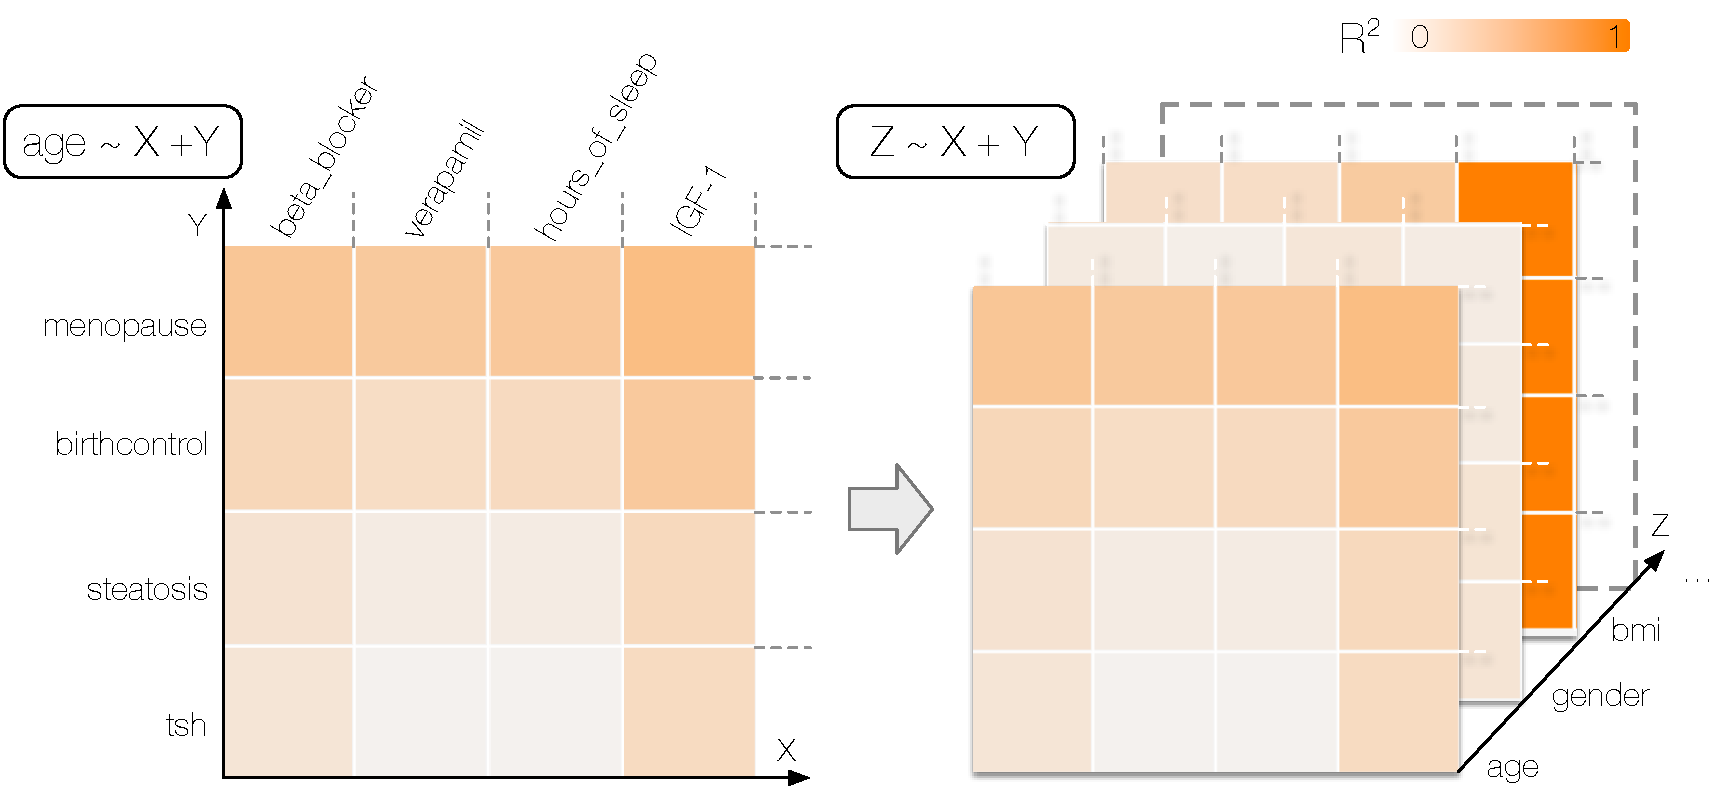
\includegraphics[width=3.5in]{figures/cube}
 \caption{
 (left) Overview visualization using a mosaic plot for the formula $Z \sim X + Y$, where $Z$ assumes feature $Age$.
 %%
 The $R^2$ values extracted from the regression formulas depict the goodness of fit and are mapped to color saturation.
 %%
 A saturated color shows a strong correlation.
 %%
 (right) Since $Z$ assumes all features $n$ as given by the formula, it yields $n$ mosaic plot visualizations.
 %%
 These represent the slices in our cube.
 %%
 The $R^2$ values of each slice voxel is mapped on opacity in the 3D-view later on, reducing the occlusion of other values.
 }
  \label{fig:Cube}
\end{figure}
%%
The goal of an overview visualization is to provide a comprehensive view on the data (raw or using descriptive metrics \cite{Bertini}), which is easy to understand.
%% TODO: Cite another paper here!
As described in our previous work \cite{Klemm2014VIS}, correlation values scaled between 0 (no correlation) and 1 (perfect correlation) can be encoded using color on a mosaic plot.
%%
Regression models are more complex, having many associated describing metrics.
%%
For the \emph{Regression Cube} analysis we are interested in the goodness of fit of the resulting model, which allows to infer about the predictive quality of the independent features included in the model.
%%
As described in Section~\ref{sec:RegressionAnalysis}, the $R^2$ value is the metric allowing for this kind of assessment.
%%
\paragraph{2D (Slice) View.}
%%
Since $R^2$ is scaled between [0,1], it allows for comparison between regression models.
%%
We can apply the same mosaic plot mapping by translating the $R^2$ values to color saturation (Fig.~\ref{fig:Cube} a).
%%
This describes a 2D regression square for dynamic variables $X$ and $Y$ (e.g. $Age \sim X + Y$).
%%

\paragraph{3D (Cube) View.}
%%
Introducing $Z$ creates a 3D \emph{Regression Cube} (Fig.~\ref{fig:Cube} b).
%%
$R^2$ values of each cube entry (\emph{voxel}) is mapped to opacity to reduce the overlap.
%%
The visualization of $R^2$ values derived from different regression cubes (e.g. $Z \sim X + Y$) is misleading, as they can be compared relatively, but not in precise numbers.
%%
Therefore, the $R^2$ results of different regression methods are encoded using different colors (e.g. blue for linear regression and red for logistic regression).
%%
This way, the cube can easily be extended using other regression types.
%%
For cubes having one fixed target feature, such as $Cancer \sim X + Y + Z$ no such encodings are required and the $z$ dimension can be compared directly.
%%
\\\\
Our goal is to create an overview visualization for a data set, but on the other hand we also want to incorporate expert knowledge into the visualization by adapting the underlying formulas.
%%
These two approaches do not exclude each other, they rather underline the difference in purpose of the chosen formula.
%%
Different analysis approaches require different starting points using the \emph{Regression Cube}.

\subsection{Analysis Workflow} \label{sec:Workflow}
%%
\begin{figure}[htb]
 \centering
 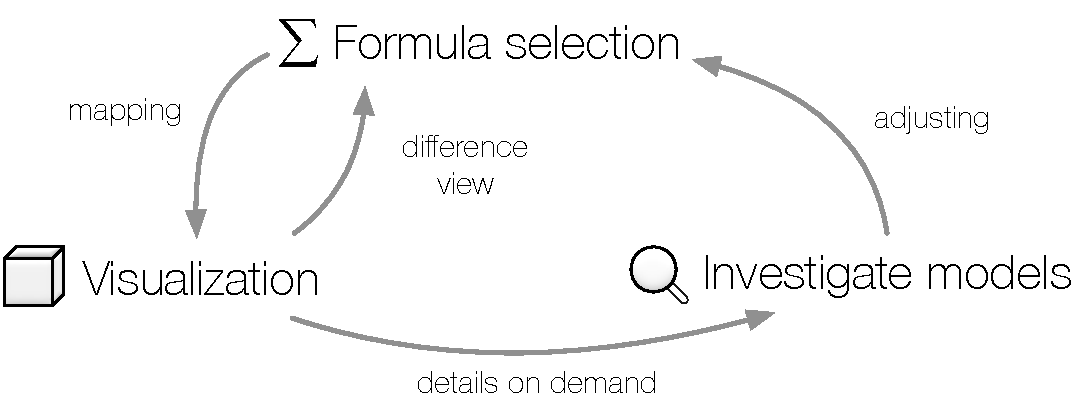
\includegraphics[width=3.0in]{figures/workflow}
 \caption{
 Workflow of the analysis using \emph{Regression Cubes}.
 %%
 % The analysis starts with a set of features given by the data set.
 %%
 [\textbf{1.AF}] The workflow starts by declaring formula regarding to specify a hypothesis, or use a predefined formula for a hypothesis-free analysis.
 %%
 [\textbf{2.SI}] The \emph{Regression Cube} is then visualized.
 %%
 The user has the option to either adjust the formula or to derive details on demand on a specific regression.
 %%
 [\textbf{3.ZF}] Insights into the data yield either an adjustment of the current formula or selecting a difference view.
 %%
 The latter is used to compare regression cubes.
 %%
 [\textbf{4.DD}] Details about features using the 2D mosaic plot representation yields insights and hypothesis about feature relations.
 }
  \label{fig:Workflow}
\end{figure}
%%
%\com{Different Formulas work as different steps in the analysis (Fig.~\ref{fig:Workflow})}
%\com{Workflow for different analysis approaches.}
%\com{0. Select the Variables.}
%\com{1. Select the Formulas}
%\com{a) Analysis without hypothesis about the data set (z ~ x+y)}
%\com{b) Analysis without hypothesis with confounder (z ~ age)}
%\com{c) Analysis with hypothesis about the data set (Var ~ x+y+z)}
%\com{d) Use Difference View}
%\com{d) Clarify using confounder (Var ~ x)}
%\com{3. Find interesting pane.}
%\com{4. Get Details on Demand.}
%%
The analysis workflow follows the Visual Analytics (VA) Mantra of Keim et al. \cite{Keim}:

\textbf{Analyze First} [\textbf{1.AF}]. Choosing an initial regression formula triggers the \emph{Regression Cube} calculation on the given data set, filtering the dimensions of the dependent feature through the CFS algorithm.

\textbf{Show the Important} [\textbf{2.SI}]. The 3D-cube visualization acts as an overview over the whole data set.
%%
Regression models with large $R^2$ values can be spotted here fast, steering the users attention to the respective slice.

\textbf{Zoom, Filter and Analyze Further} [\textbf{3.ZF}]. The slices of interest can then be analyzed using the 2D mosaic plot of the slice.

\textbf{Details on Demand} [\textbf{4.DD}]. Precise information about the individual regression models (coefficients, associated confidence intervals and p-values) can be retrieved based on the data point representatives (e.g. in a hover-modal on a currently selected data point).
\\\\
We use the squared bracket abbreviation for each step to denote the affiliation the system design section later on.
%%
As seen in Fig~\ref{fig:Workflow}, the workflow is highly iterative.
%%
Observations in the 2D-mosaic plot or simply the CFS-based features can trigger new analyses by adjusting the underlying regression formulas.
%%
This can be carried out either to refine the current formula based on observations, or creating a new regression cube for a difference view.
%%
\paragraph{Hypothesis-Free and Hypothesis-Based Analysis.}
%%
Input formulas reflect \emph{hypotheses} about the data.
%%
Using the operators, dynamic variables and dataset features, many different assumptions can be formulated.
%%
To support \emph{hypothesis-free} analysis we provide a default formula:

$Z \sim X + Y$.
%%
This cube represents all possible combinations of two independent features towards all features in the data set, since we do not know which feature(s) are of interest.
%%
Each slice represents a different target feature.
%%
It is therefore suitable for an explorative analysis to give a general impression about relationships in the data set.

Hypotheses about the data are reflected in either how dynamic variables are related using the regression operators.
%%
Also, static features can be added for each regression formula.
%%
Here are a few examples:

%%
$Cancer \sim X + Y + Z$ is an example for the formulation of a hypothesis, where a specific feature is analyzed.
%%
All combinations of three independent features towards the target are analyzed through the cube.

$Cancer \sim X + Y + Z + feature_1:feature_2$ encodes more assumptions.
%%
This formula models the hypothesis of an interaction between $feature_1$ and $feature_2$ (denoted with $:$) being relevant for the target feature, but it is not clear how other feature combination influence the result.
%%
Therefore, the cube incorporates this interaction for all $X$,$Y$ and $Z$ values as independent features.
%%

$Cancer \sim X + Y + Z$ subtracted with the $R^2$ from $Cancer \sim Age$ excludes the confounding effect age has towards the target $Cancer$ feature.
%%
This is achieved through cube comparison.
%%

\paragraph{Cube Comparison.}
%%
Regression Cubes can be compared by creating difference views.
%%
One cube (formula) acts as reference.
%%
The absolute difference in $R^2$ values towards the second cube is calculated, yielding a difference cube showing only the differences between the two formulas.
%%
It can for example be utilized for comparing the influence of one feature towards the complete result (e.g., $Z \sim X + Y$ and $Z \sim X + Y + Income$)
%%
% \paragraph{Formula Types.}
% %%
% Input formulas reflect \emph{hypotheses} about the data.
% %%
% Using the operators, dynamic variables and dataset features, many different assumptions can be formulated.
% %%
% Here we show just a few examples on how formulas can serve different purposes.
%
% $Z \sim X + Y$ is the default formula.
% %%
% This cube represents all possible combinations of two independent features towards all features in the data set, since we do not know which feature(s) are of interest.
% %%
% Each slice represents a different target feature.
% %%
% It is therefore suitable for a \emph{hypothesis-free} explorative analysis to give a general impression about relationships in the data set.

\section{System Design} \label{sec:SystemDesign}
\begin{figure}[htb]
 \centering
 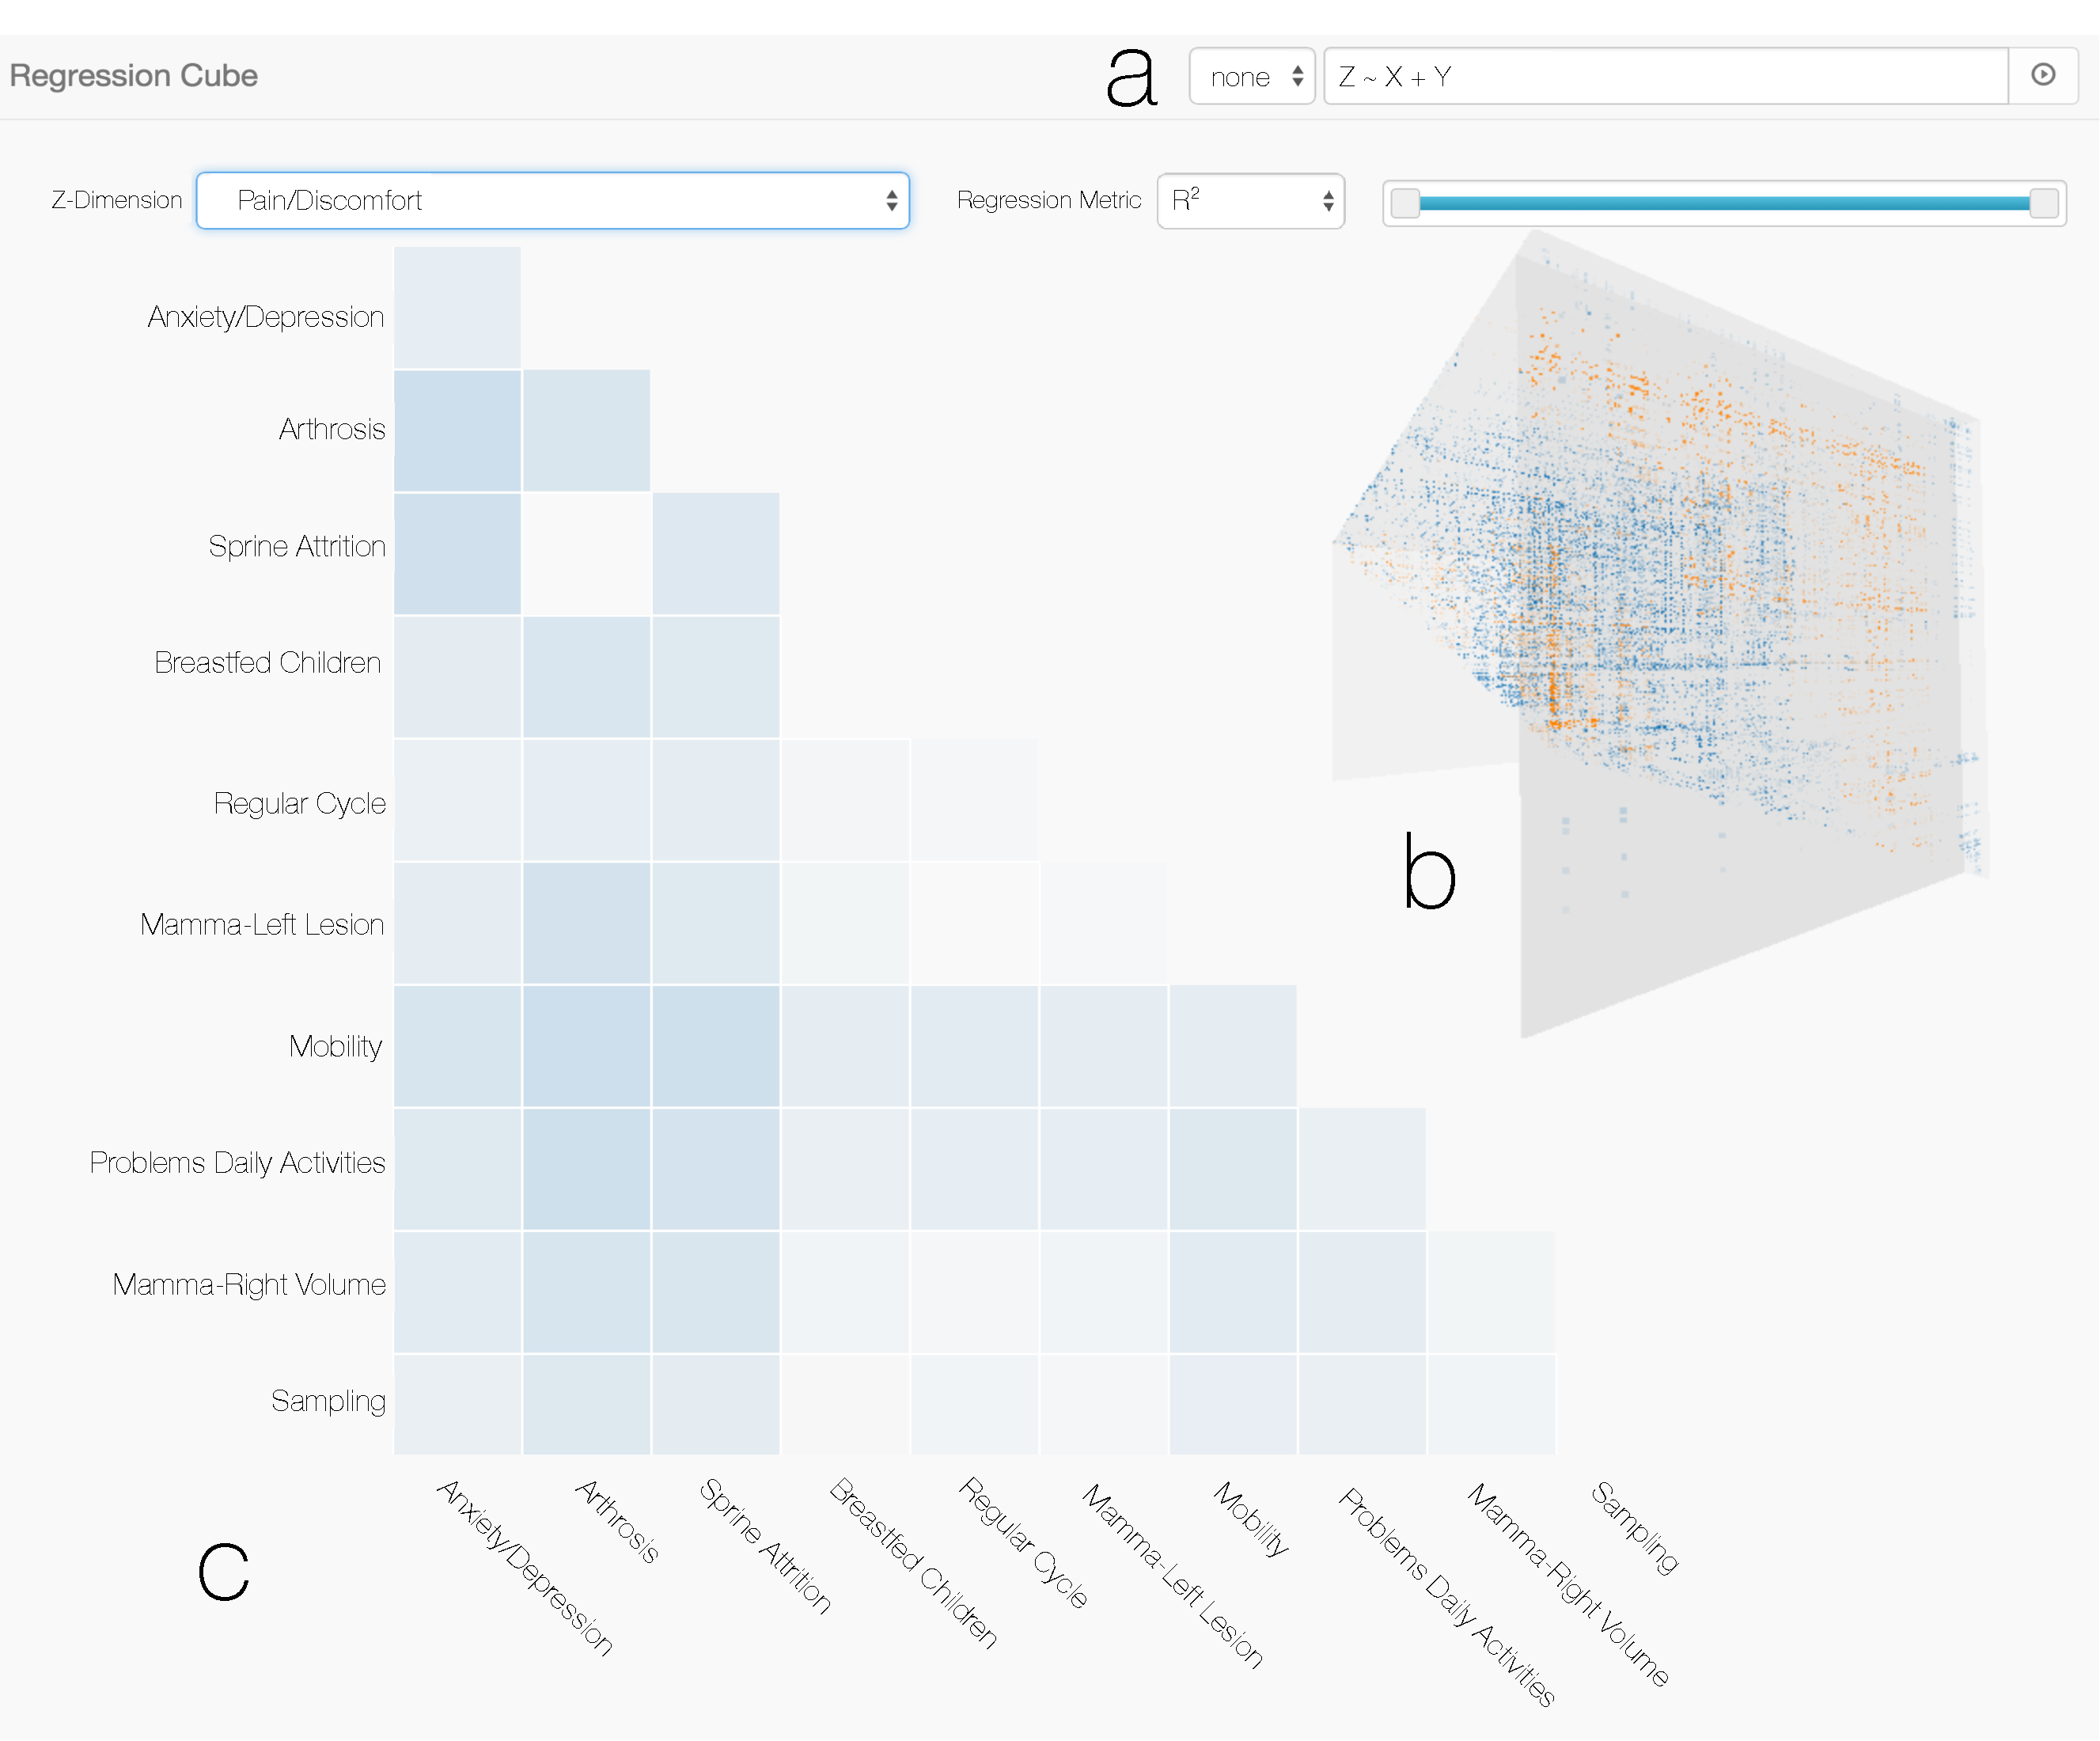
\includegraphics[width=3.5in]{figures/system}
 \caption{
 %%
 Breast fat data set loaded into the \emph{Regression Cube} prototype.
 %%
 (a) Using the formula input, the user specifies the dependent feature as well as its calculation rules.
 %%
 (b) 3D cube visualization, showing values above the cube matrix diagonal as overview.
 %%
 The values of the currently selected slice are mirrored and represented as orange data points on the slicing plane.
 %%
 (c) 2D mosaic plot visualization of the selected slice for feature \emph{Pain/Discomfort}.
 %%
 %\com{TODO: Adapt formula to final image.}
 %%
 %Context information is shown for the regression model of $Parenchym \sim Bronchitis + AlcoholLast30Days$, depicting details about the confidence intervals, coefficients and associated p-values.
 %%
 %\com{Screenshot of the cube visualization embedded in the framework}
 %\com{Also include active tooltip}
 }
  \label{fig:System}
\end{figure}
%%
We designed our system with openness and ease of use in mind.
%%
Using open formats as input interfaces does not restrict the application towards non-epidemiological data sets.
%%
The focus lies on creating an overview visualization and gaining insight into relationships into the data, which triggers further analyses (maybe with other (statistical) tools).
%%
Therefore, the system has to be intuitive and comprehensive in order to be adapted by domain experts.
%%
\\\\
% \subsection{Design and Visualization Techniques}
%%
\noindent Design choices and spaces are restricted by the underlying technologies and devices.
%% TODO: Umschreiben
Resting collaboration and exchange about data and methods on web-based technologies shows promising results, as there is no set-up time involved and domain experts can use the methods from any computer connected with the web.
%%
Web technology is by design based on a client-server architecture, making it easy to outsource computationally heavy tasks on server-clusters and transferring results to the client device.
%%
The design space spanned by web-technologies is different to standard WIMP-applications: right click menus, modal windows and menu bars are not established UI components in this context.
%%
Therefore, we have to adapt our design respecting the affordances of web pages.
%%
\subsection{System Paradigm and Components}
%%
The \emph{Regression Cube} design focuses on a clean interface, reducing the amount of user-interface elements as much as possible.
%%
This allows for a fast learning of the individual system parts.
%%
%More importantly, it allows the user to focus all mental resources on the analysis tasks, rather than wrangling with configuring the system to serve the current task or hypothesis.
%%
Our prototype consists of three components:
\begin{itemize}
	%%
	\item The \emph{file upload} section starting the analysis with providing a comma separated value (CSV) file [1.AF].
	%%
	\item The \emph{cube visualization} consisting of the 2D-mosaic view as well as a 3D-representation of the whole cube [2.SI].
	%%
	\item The \emph{formula editor} allows to adjust the formula w.r.t. a hypothesis or conducting a \emph{hypothesis-free} analysis.
	%%
	It also allows to select a reference formula for creating a difference-cube [3.ZF].
	%%
\end{itemize}
%%\com{Focus on simplification and ease of use, reducing the number of UI elements as much as possible (Statistical Visualizations often tend to put all information and settings at once to the user, which is overwhelming for the user).}
\paragraph{File-Upload and Classification [1.AF].}
%%
Popular analytics tools, such as WEKA \cite{WEKA}, owe their popularity to their support of open file types.
%%
To allow other users even outside the epidemiological application domain to access to our tool, we use standard ASCII-based CSV files.
%%
The first line in a CSV file represents all features (columns) of the data set.
%%
Each line after that represents one subject (row) and their feature manifestations.

\textbf{Classification.}
%%
Encoding variable types in CSV files is not standardized.
%%
We, however, need to ensure the correct variable type classification and have to enforce some basic standards.
%%
All categorical values have to be enclosed by quotation marks.
%%
Continuous variables are denoted as digits without enclosing quotation marks.
%%
This seems obvious, but in fact many cohort study data sets encode categorical features using ID-values, which are denoted in a data dictionary.
%%
Variables with only two manifestations are classified as dichotomous, leading to three possible data types: numerical, categorical and categorical/dichotomous.
%%
Missing values are denoted by using no character at all, a whitespace, or an empty quotation mark encapsulated string.

\textbf{Data Security.}
%%
Security issues are raised by uploading data into an online service, such as our prototype.
%%
The use of epidemiological data is preceded by a detailed description of the analysis purpose and has to be approved by ethics committees.
%%
Preventive steps have to be taken to restrict access to unauthorized subjects.
%%
%We decided against a user account system because it reduces the ease of use largely without having a direct advantage for the user.
%%
We apply a SHA-256 hashing on the data set name using the data contents and disable directory listings on the web server to avoid data set downloads.
%% TODO: Implement this
Data sets are deleted from the server after closing a session.

\paragraph{Formula Editor [1.AF, 3.ZF].}
%%
After uploading the data, the user can specify a formula or use the default ($Z \sim X + Y$).
%%
Entering a formula is provided via text input.
%%
On formula input, a context modal displays all data set variables, as well as the available operators and their function.
%%
This allows to comprehend the function of the underlying formula for users without statistical background about regression analysis and its notation.
%%
Auto-completing input variables also simplifies the approach and also works as spell-check of variable names.
%%

\textbf{Formula Validation and Calculation.} The formula is checked for validity directly on input.
%%
The text input containing the formula is marked using a red halo to indicate invalid input, which turns green for valid formulas.
%%
This prevents processing errors on the statistical processor back-end.
%%
Confirming a formula triggers the cube calculation, which is preceded by determining all required formulas.
%%
These are then divided by the number of available statistical back-end processors available, driving a \emph{cloud-computing}-based approach.
%%
In theory, the calculation duration is reduced by a factor of $0.5$ by every statistical processor.
%%
In praxis, data transmission and differences in machine specifications always influence the speed.

%%
\textbf{Difference-Cube.}
Adding a formula also adds it to the reference selection for a difference cube.
%%
Since all cells in the cube are represented using $R^2$ values, a difference cube is calculated by denoting the absolute difference of $R^2$ for each cell.
%%
%%If the user selects a reference formula, the absolute difference of $R^2$ values between the cube described by the reference and the currently active formula are calculated and shown.
%%

%\com{Dynamic Type Checking, Auto-Completion Analysis Trigger, Comparison between Cubes, triggering of cube calculation, parallelization of formula calculation}

\subsection{Regression Cube Visualization [2.SI].}
%%
The visualization and interaction with the \emph{Regression Cube} is the prototype core.
%%
Results from the statistical processors are uploaded into the visualization slice by slice, allowing the assessment of the data as soon as parts of the calculations are finished while the rest is still in processing.

\paragraph{Usage of a Regression Prism for information reduction.}
%%
Figure~\ref{fig:Cube} shows that all values are mirrored along the diagonal of the mosaic plot matrix.
%%
This is due to the symmetry of basic regression operators.
%%
$Z \sim X + Y$ produces the same result as $Z \sim Y + X$.
%%
Therefore we can discard half of the results to reduce visual clutter and repetition, yielding a \emph{Regression Prism}.
%%
This opens up space for displaying additional information.
%%
Along the diagonal, $X$ and $Y$ assume the same feature, $Z ~ X + Y$ turns into $Z ~ X$ because the regression automatically ignores doublings.
%%
The diagonal therefore acts as reference on how strong the correlation for the given row (or column) feature is.

\paragraph{3D-Prism as Data Mini-Map.}
\com{Add section about difference view for static target features.}
%%
The 3D-cube representation acts as an overview over the whole data set, but its purpose is not to derive detailed information about data points.
%%
It serves an function similar to a mini-map, guiding the attention towards points of interest in the data, as well as giving context information about adjacent data values when using the 2D mosaic plot.
%%
It serves the purpose of \emph{Show the Results} after the \emph{Analyze First} step in Keim's VA-Mantra.
%%
The displayed prism shows values above the matrix diagonal.
%%
%% TODO: Add reference for disadvantages of 3D information visualizations!
\paragraph{Tackling the disadvantages of 3D information visualization.}
3D-Information visualizations are often criticized for introducing occlusions and interaction problems, which often do not balance out the advantages of using the third dimension for visual mapping.
%%
We aim to minimize these problems as much as possible.
%%
Since the $R^2$ values are mapped on data point opacity, only large values are highlighted in the prism, guiding the focus to the respective slices.
%%
It also creates a very sparse representation, since the majority of regression models yield (depending on the data set and the chosen formula) low $R^2$ values.
%%
Also, the preceding correlation based feature selection reduces the information space significantly, leading to sparse cubes.
%%
Overlapping is still an issue, but this way greatly reduced in its affect to the readability of the visualization.
%%

%% INTERACTION
Rotating with the cube is restricted to the y-axis, preserving the mental map to position individual features.
%%
The cube is always oriented according to the 2D-representation, allowing for an easy mental combination of the two representations.
%%
Allowing more degrees of freedom was confusing to our users and also did not add value to the visualization.
%%
We provide also a zoom functionality using the mouse wheel input.
%%
%\\\\
\paragraph{Cube Slice Selection [3.ZF].}
%%
In order to \emph{Zoom, Filter and Analyze Further}, the user has to navigate towards different slices of interest.
%%
We propose two ways to achieve this.
\begin{itemize}
	\item \emph{Applying the slicing metaphor from 3D volume data.}
	%%
	In medical volume data renderings, slicing views very common to view details on a selected plane in the scene.
	%%
	We employ this technique for selecting cube slices (e.g. by moving a plane via vertical mouse input while pressing the right mouse button).
	%%
	We, however, still display the whole 3D-object instead of cutting away information towards the slice position.
	%%
	\item \emph{Selecting the slice using a dropdown menu} provides fast access to plane selections when the user already knows the slices of interest.
	%%
\end{itemize}
%%
The currently selected slice is denoted with a semi-transparent gray plane.
%%
The space available from visualizing only the prism generated from the upper half of the cube diagonal is used to display information about the current selected plane.
%%
the values are projected on this plane to give an overlapping-free view on the data points, which makes it easier to identify the current slice.
%%
%It also allows for a fast slicing through the cube and assessing the information.
%%
%\com{display of skewed cube, combination of 2D to 3D, navigating between the two views, projection of current slice to the 3D-Cube, details on demand}
%\\\\
\paragraph{2D Mosaic Plot Slice Visualization [4.DD].}
\com{Add Figure reference!}
%%
The 2D mosaic visualization shows all values below the matrix diagonal of the current slice, creating optical equivalence towards the 3D cube.
%%
To reduce visual clutter, the 2D view only shows dimensions, which are retrieved through the correlation based feature selection.
%%
The free space above the matrix diagonal is used to display the 3D cube.
%%

The purpose of this view is the detailed assessment of the underlying regression models.
%%
By hovering over a data entry in the plot, a tooltip model displays detailed information about a models coefficients, associated $p$ values and confidence intervals.
%%

%\com{Simplicity of interface to allow for steep learning curve.}
%\com{Visualization as skewed cube to reduce visual clutter and remove double entries.}
%\com{Cube acts as visual mini map to give a global impression over the data.}
%\com{current pane shown using a heat map visualization.}
%\com{details on demand for selected regression formula.}
%\com{comparison view using reference cubes.}

\section{Implementation} \label{implementation}
\begin{figure}[htb]
 \centering
 \includegraphics[width=3.5in]{figures/implementation}
 \caption{
 The front-end (left) is written in \emph{HTML5}/\emph{CSS3}/\emph{Javascript} and uses different Javascript libraries, such as \emph{Angularjs}, \emph{Three.js} and D3js.
 %%
 The web-server back-end (right) is written in \emph{Nodejs}, hosting is carried out using \emph{Heroku}.
 %%
 \emph{R} and \emph{OpenCPU} constitute the statistical back-end (top) to compute the \emph{Regression Cubes}.
 %%
 Additional statistical back-ends can be attached to the system to decrease the computation time.
% The number of attached machines to the system 
%    the  the  Describe the Bootstrap/Angular/D3 Frontend, Node backend, R/OCPU Backend.}
 }
  \label{fig:Implementation}
\end{figure}
%%
% Using web technologies for prototyping allows for:
% \begin{itemize}
% 	\item easy exchange of software, without the need of installing anything other than a modern web browser,
% 	\item fast iterative adaption of method changes, without the need of installing updates,
% 	\item outsourcing computation-heavy tasks to server-clusters, which do not have to be in local proximity.
% \end{itemize}
% %%
%%
We rely on web-based technologies for our prototype.
%%
The ongoing transition of open-science software into the web spawned numerous projects, making state-of-the-art algorithms available in this domain.
%%
\paragraph{Front-End.}
%%
The front-end is created using \texttt{HTML5}, \texttt{CSS3} and \texttt{Javascript}.
%%
\texttt{Angular.js}\footnote{Open Source; Maintained by Google, \href{https://www.angularjs.org/}{\texttt{angularjs.org}}} abstracts web application into models and views, allowing for a responsive way to combine \texttt{HTML} and \texttt{Javascript}.
%%
\texttt{Angular.js} is forcing developers to write modularized code, which makes the components easier expandable while keeping the code maintainable by including unit tests.
%%
The page layout is handled using \texttt{Twitter Bootstrap}\footnote{Open Source; Maintained by Twitter, \href{http://getbootstrap.com}{\texttt{getbootstrap.com}}}, which also provides a rich set of UI elements with proper stylings.
%%
The 2D mosaic plot is implemented using \texttt{Data driven Documents} (\texttt{D3.js}), which is popular in information visualization using vector graphics \cite{D3}.
%%
It provides fast and easy methods for binding data to graphical elements.
%%
The 3D plot is created using the WebGL-based \texttt{Threejs}\footnote{Open Source; Originally developed by R. Cabello, \href{http://threejs.org}{\texttt{threejs.org}}} library.
%%
We experimented with different ways for achieving the cube representation, including volume rendering, cube primitives for each data point and shader-based solutions.
%%
Open source volume rendering methods are available but do not satisfy our requirements.
%%
Creating a cube primitive for each data point resulted in non-interactive frame-rates for data sets larger than 30 features (creating 30$^3$ cube primitives).
%%
We use a shader-based solution by rendering the cube as a sprite based particle system, allowing to customize color and opacity of every data point.
%%
It also is the fastest solution that we tested.

\paragraph{Back-End.}
Two server structures serve as back-end.
%%
The first one is the web-server, which is written in \texttt{Javascript} using \texttt{NodeJS}\footnote{Open Source; Maintained by Joyent Inc, \href{http://nodejs.org}{\texttt{nodejs.org}}}, running on Googles V8 Javascript runtime environment.
%%
It is hosted on \texttt{Heroku}\footnote{Owned by Salesforce.com, \href{https://www.heroku.com/}{\texttt{heroku.com}}}, a cloud application platform.
%%

The statistical processors yield the second structure.
%%
They rely on the statistical programming language \texttt{R}.\footnote{Open Source; \href{http://r-project.org}{\texttt{r-project.org}}}
%%
It is widely adopted in the statistical analysis community, yielding a rich support of fast state-of-the-art statistics algorithms as well newly published methods.
%%
\texttt{OpenCPU} is a \texttt{R} package and provides a API for accessing it via HTTP calls \cite{Ooms}.
%%
This way, any computer, which runs \texttt{R} can be turned into a statistical processor for our project.
%%
The back-end functions necessary for all cube calculations are provided via an \texttt{R} package.
%%
It uses multi-core optimization to use all machine CPUs to speed up the calculation process.
%%
The server workload balances are managed by the front-end code.

\paragraph{Access and Source.}
%%
A running instance of the \emph{Regression Cube} prototype can be found under \href{http://regressioncube.herokuapp.com/}{\texttt{regressioncube.herokuapp.com}}.
%%
The source for the prototype is freely available at \texttt{Github}.\footnote{\texttt{R}-based back-end: \href{https://github.com/paulklemm/regression-cube-r-package}{\\\texttt{github.com/paulklemm/regression-cube-r-package}}}$^{,}$\footnote{Front-End and Nodejs Webserver: \href{https://github.com/paulklemm/regression-cube-prototype}{\texttt{\\github.com/paulklemm/regression-cube-prototype}}}
%%
Instructions and code on how to create a setup running the \emph{Regression Cube} statistical back-end through a \texttt{Ubuntu} server using \texttt{OpenCPU} are referenced in the repository.
%%
The front-end can be deployed using \href{https://www.heroku.com/}{\texttt{www.heroku.com}} by cloning the repository into a Heroku homepage. 
%%
%The front-end source as well as the \texttt{Nodejs} backend can be found here: .
%%
% \com{Use VAST'14 as Guideline}
% \com{Cloud computing}
% \com{Volume Rendering vs Particles}
% \com{Speed is merely a matter of available server machines due to parallelization process.}
% \com{Security enabled by hashing files.}
% \com{Bootstrap/Angular/D3 Frontend, Node backend, R/OCPU Backend (Fig.~\ref{fig:Implementation})}

\section{Application} \label{application}
%%
\begin{figure*}[htb]
 \centering
 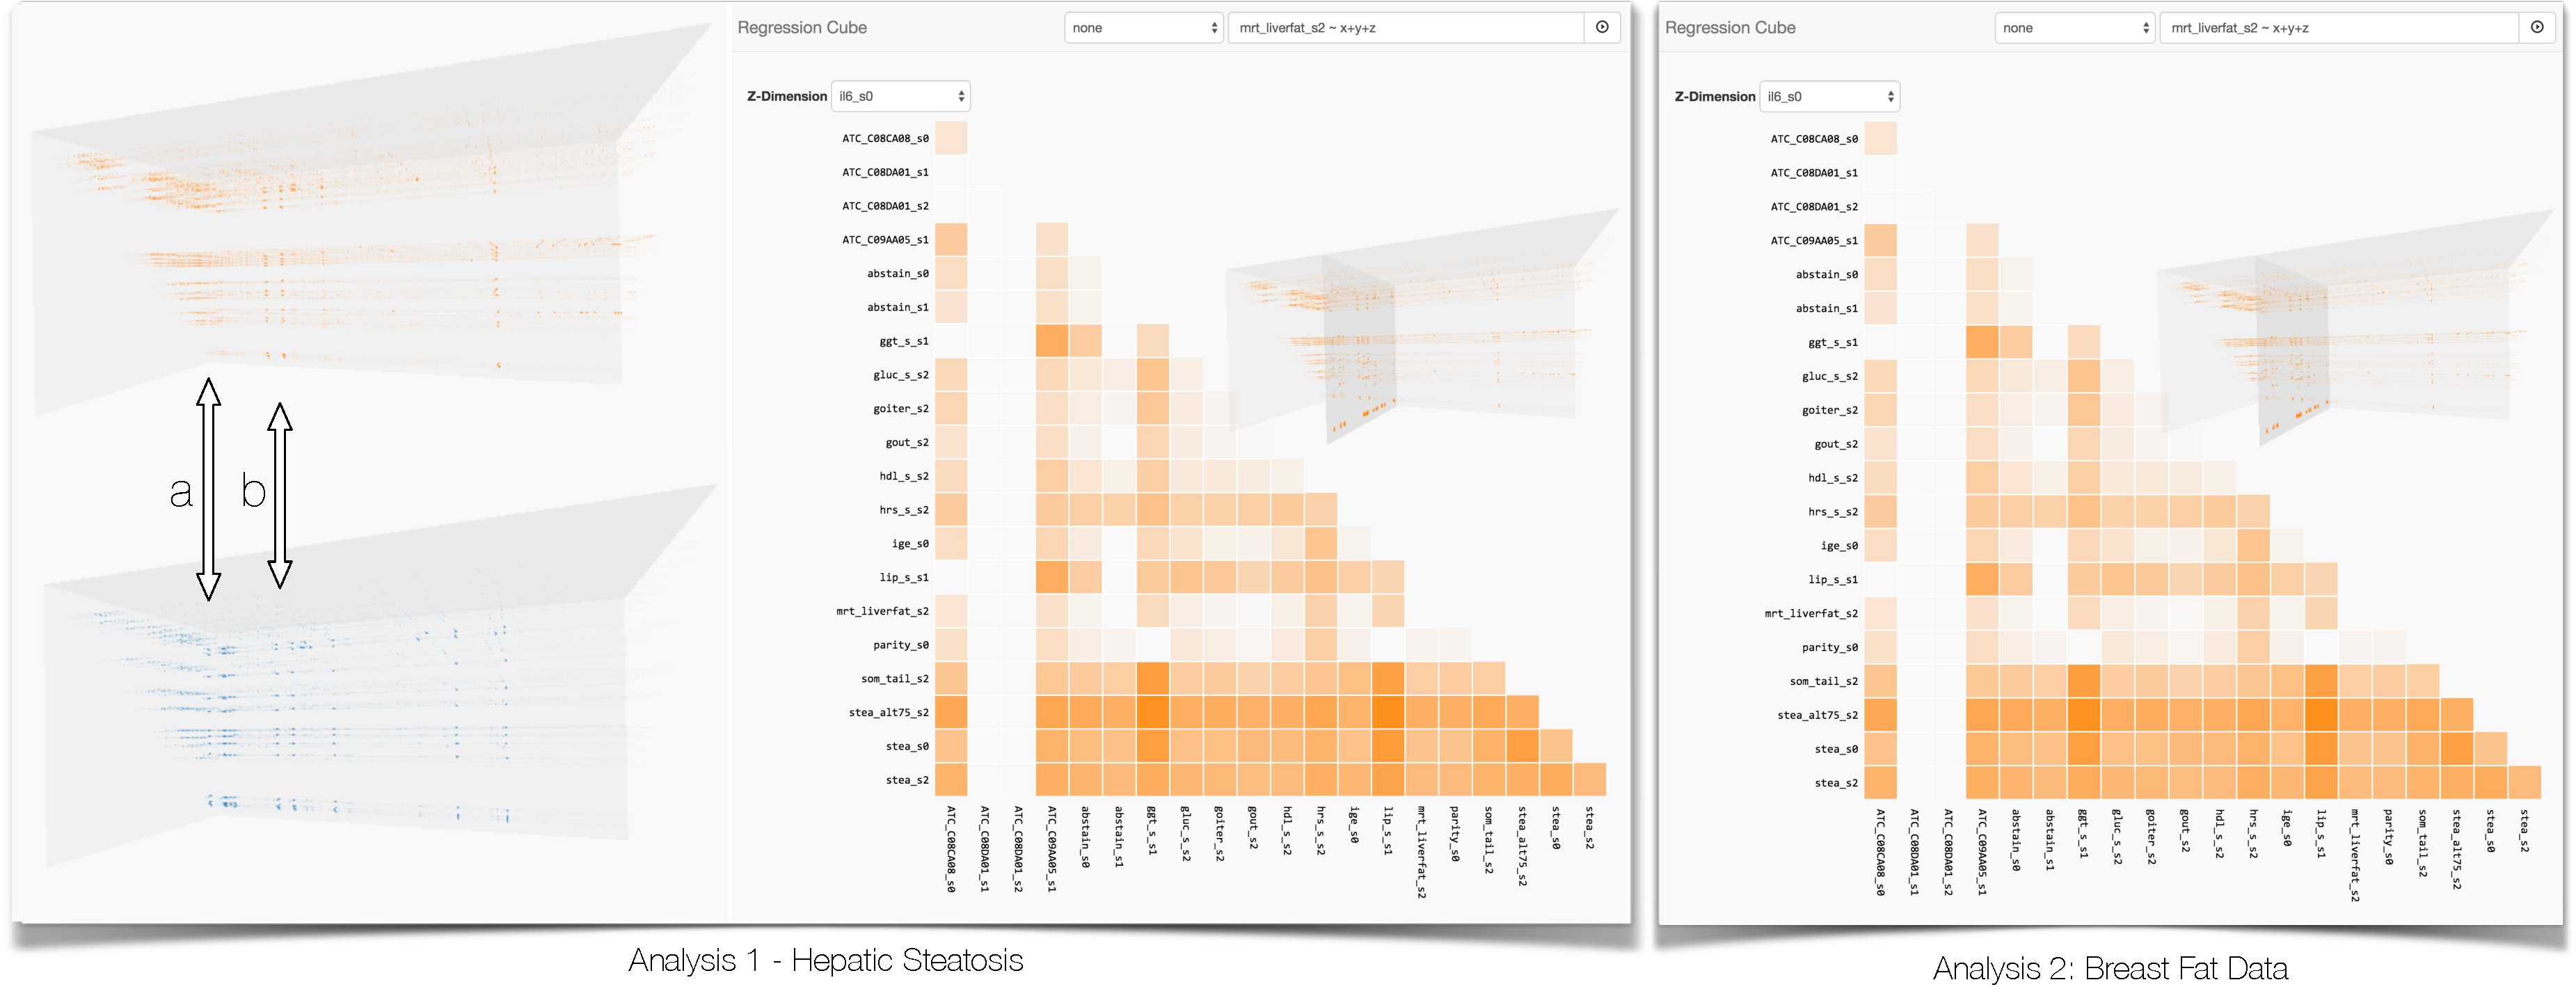
\includegraphics[width=7.0in]{figures/application}
 \caption{
 The analysis of the numerical and dichotomized target feature depicting liver-fat values yields similar results (left).
 %%
 In (a), hotspots for somatometrical features with high correlations were found.
 %%
 High correlations were also found for features depicting \emph{hepatic steatosis} (b).
 %%
 A high correlations between \emph{Interleukin-6}, \emph{hepatic steatosis}, \emph{GGT} and \emph{Lipase} (highlighted using arrows) was found during the analysis using the 2D mosaic plot.
 %%
 \com{Caption Breast Fat Data}
 }
  \label{fig:Application}
\end{figure*}
%%
In this section, we describe how we applied the \emph{Regression Cube} to two epidemiological data sets.
%%
The hepatic steatosis data set was analyzed using data mining algorithms, yielding risk groups, which we now analyze further.
%%
Also, we try to reproduce the prior results from this analysis as proof-of-concept of our method.
%%
The breast fat data set is the foundation for an explorative analysis towards the influencing parameters of the parenchyma tissue of the female breast.
%%

Both data sets are unusual for epidemiological analysis regarding their feature extent.
%%
Usually, only a few features depicting a hypotheses are compiled into a data set to assess them using statistical tools.
%%
The herein used data sets comprise several hundred features.
%%
Our method focuses on data exploration and knowledge extraction and requires a wide scope of sociodemographic, medical and lifestyle features.
%%
\subsection{Participants, Setup and Procedure}
%%
To assess the ability of a system to discover knowledge is difficult to measure.
%%
Lam et al. \cite{Lam2012} propose the \emph{Visual Data Analysis and Reasoning} (\emph{VDAR}) technique, which is focused on the characterization of a systems' ability to generate hypotheses and explore the data in order to extract information.
%%
\emph{VDAR} can be carried out using case studies using thinking-aloud techniques to comprehend the reasoning and thought process of the user.
%%
\paragraph{Participants, Setup and Procedure.}
%%
%One major advantage of focusing on web-based research was the possibility to bridge the geographical gap towards the epidemiological domain experts.
%%
We conducted a web-based analysis by using an online-meeting software, which features voice chat as well as screen sharing.
%%
Starting an analysis using these techniques take about 5-10 minutes of setup time.

The sessions started with an initial overview of the system, showcasing its features and functionality.
%%
After that the experts use the system on their own computers.
%%
The screen-sharing function was still used to observe the actions of the expert.
%%
All sessions were video recorded to be processed later on.
%%

%%
We conducted a study with two participants, who also co-authored this publication.
%%
Domain expert for the breast fat data set analysis is KH, a clinician (10 years of experience) with focus on epidemiological research.
%%
\emph{KH} is a radiologist, responsible for the SHIP-MRI acquisition and also responsible of the mammography analysis.

The hepatic steatosis data set is analyzed by \emph{UN}, a data scientists responsible for prior analysis of the data with.
%%

\emph{TI}, a statistician with focus on epidemiology (\com{TODO} years of experience) assesses the statistical reliability of the tool and the underlying methods without a focus on a specific data set.
%%
\subsection{The Breast Fat Data Set}
The breast fat data set was compiled to find associations between parenchyma tissue proportion in the female breast towards other features in the data.
%%
The ratio between parenchyma and cellular connective tissue (breast density) has been shown to be associated with breast cancer.
%%
Studies describe a four to five times increased risk of getting breast cancer for participants with a breast density above 50\% \cite{Mccormack2006}.

The data comprises 1.186 subjects (368 from \texttt{SHIP-2}, 818 from \texttt{SHIP-TREND-0} cohort).
%%
It contains 231 dimensions, holding information about
\begin{itemize}
	\item \emph{somatometric features}, e.g., body size, weight or BMI, 
	\item \emph{lifestyle features}, e.g., alcohol/tobacco consume, 
	\item \emph{personal history}, e.g., occupation, marital status,
	\item \emph{medical history}, e.g., current or prior diseases or laboratory values, such as cholesterol levels,
	\item \emph{women specific features}, e.g., number of born children, contraception type or hormone replacement therapy and
	\item \emph{mammography features} derived from the image data.
\end{itemize}
%%
The latter were derived using a level set based segmentation \cite{Ivanovska2014} of MRI image data for each subject.
%%
\com{Check this with Mrs. Hegenscheid, probably most of them were segmented by hand!}
%%
%\com{Describe Parenchym tissue and its relation to breast cancer.}
%\com{Describe how the data was acquired and preprocessed}

The data of each cohort was presented as individual \texttt{SPSS} files.
%%
All data related to the mammography was stored in a additional file.
%%
We converted the \texttt{SPSS} data sets to CSV and used \texttt{R} to merge the data sets together using their ID.
%%
All features were renamed to be expressive, e.g., \emph{chro\_09a} is now denoted as \emph{Disease\_Osteoporosis}.
%%
This avoids the need of defining a separate data dictionary file for the \emph{Regression Cube}, translating the feature names.
%%
All male subjects were removed as their data does not contribute to the analysis.
%%
\subsection{The Hepatic Steatosis Data Set}
We employ a subset of the data set which was used in \cite{Niemann2014} to identify predictive features with respect to the reversible disorder hepatic steatosis (fatty liver).
%%
The binary target feature is derived from the liver fat concentration which was measured with Magnetic Resonance Imaging (MRI).
%%
In particular, participants with a liver fat concentration of no more than 10\% are mapped to the 'negative' class; values greater than 10\% are mapped to the 'positive' class.
%%
The data set contains labels for 578 participants for which the MRI data was available to that point.
%%
Note that MRI was performed only in SHIP-2, so the target feature is present for just one of three study waves.

%%
Apart from the target feature, the data set contains 199 features extracted from participants' questionnaire answers and medical tests.
%%
They are features on socio-demographics (sex, age, etc.), features on consumption behavior (e.g. alcohol and cigarettes), SNPs, features extracted from laboratory data (e.g. sera concentrations), and two features on the results of the liver ultrasound.
%%
The names of 85 features have the suffix \emph{s0} meaning that their values have been recorded in SHIP-0 (first study moment), 50 features exhibit the suffix \emph{s1} and 55 features have the suffix \emph{s2}, alongside 10 time-independent SNPs.
%%

In \cite{Niemann2014}, the authors show that women and men exhibit differences in the class distribution of the liver fat concentration.
%%
Also, for women they identify that there is a association between age and liver fat concentration.
%%
They compute an appropriate cut-off value of 52 years for which the class distribution is most homogeneous within the resulting subsets.
%%
Based on this observations, we perform our analysis on three sub-populations, \emph{females}, \emph{males} and \emph{females} older than 52 years.
%%
\subsection{Case 1: Hypothesis-free Analysis of the Breast Cancer Data Set}
%%
%%
The analysis goal is to find relationships on the breast cancer data using features derived from the mammography analysis.
%%
Relationships between the share of parenchyma tissue on the overall breast volume are of high interest \cite{Mccormack2006}.
%%

\subsection{Case 2: Hypothesis-driven Analysis of the Hepatic Steatosis Data Set}
\com{Add R$^2$ values}
%%
We refer to each analysis step regarding to their belonging in the VA-Mantra (Sec.~\ref{sec:Workflow}).
%%
The analysis goal is reproducing results based on \cite{Niemann2014}.
%%
Therefore, \emph{UN} started the \textbf{AF} step using the dichotomized MRI fat liver concentration using the formula $mrt\_liverfat\_s2 \sim X + Y + Z$ for \emph{male} subjects.
%%
The \emph{SI} step using the 3D cube representations locates hotspots at the end of the cube (Fig.~\ref{fig:Application} a).
%%
\textbf{ZF} by slicing through the cube using the mouse input to inspect the hotspots using the mosaic plot (\textbf{DD}) revealed high correlations for somatometric features, hepatic steatosis indicator-features as well as laboratory values, such as creatinine (\com{important for kidney}) and uric acid (\com{gout, diabetes}) magnitudes.
%%
Similar results present for analyzing the \emph{female} groups.
%%
\emph{UN} could reproduce most results, some features features exhibit lower correlations though, e.g., creatinine magnitudes.
%%
Relationships not described in \cite{Niemann2014} were found, such as enzymes indicating liver dysfunctions, e.g. \emph{aspartate aminotransferase}.
%%
Due to the difference between our regression-model approach and the decision-tree approach presented in \cite{Niemann2014}, a complete matching set of correlating features are not expected.

% %%
% The goal at the beginning of the analysis was to reproduce results based on the prior analysis.
% %%
% Subjects with a fatty liver could be identified using somatometric features, hepatic steatosis indicator-features as well as creatinine (\com{important for kidney}) and uric acid (\com{gout, diabetes}) magnitudes.
% %%
% The analysis was started with the target feature \emph{liver fat content} (\emph{mrt\_liverfat\_s2}), which was derived from the MRI data analysis.
% %%
% \emph{UN} therefore started the calculation using the formula $mrt\_liverfat\_s2 \sim X + Y + Z$ for \emph{male} subects.
% %%
% %%
% %%
% The data set containing all \emph{males} showed broad consensus with the expected results.
% %%
% The 3D-cube showed highlighted features at the end of the cube (Fig.~\ref{fig:application} a).
% %%
% Using the mouse-slicing allowed for fast navigation to the respective features.
% %%
% They include indicators hepatic steatosis ($R^2$:XX) as well as somatometric features, such as \emph{body mass index} (\emph{BMI}) and waist circumference.
% %%
% Feature correlations with \emph{gamma-glutamyl transpeptidase} (\emph{GGT}, indicating damaged livers if elevated) were found, but with low $R^2$ of XX.
%
% %%
% UN analyzed both \emph{female} groups in the same manner, concluding with the same findings regarding \emph{somatometric} features as well as \emph{hepatic steatosis} indicators.
% %%
% Using the mosaic plot, relationships incorporating enzyme used for the diagnosis of liver dysfunctions were found, e.g. aspartate aminotransferase.
% %%
%
% For most features, UN found at least tendencies using our approach.
% %%
% Due to the difference between our regression-model approach and the decision-tree approach presented in \cite{Niemann2014}, a complete matching set of correlating features are not expected.
%
% %Regression cube calculations were carried out for

\textbf{Analysis of non-discretized target feature.}
%%
Since our method can analyze numerical target features, as opposed to decision trees used by \emph{UN} before, the analysis was conducted again for the not-dichotomized target using the same formula.
%%
The 3D-cube representation already showed generally lower $R^2$ values, but since the analysis is now based on linear regression, the $R^2$ values can not be directly compared.
%%
Correlation hot spots matched with the ones from the dichotomous target, but were generally lower ($R^2$ of XX for somatometric features as opposed to XX).
%%
We conclude that the bias introduced by dichotomizing the fat liver content enforces the findings towards liver diseases, while using the numerical features is less expressive.
%%

\textbf{Interleukin-6 correlation with liver fat.}
%%
During the analysis, one hotspot was always observed in the \emph{SI} and \emph{ZF} incorporating a high \emph{Interleukin-6} (\emph{IL-6}) correlation with liver fat values (Fig.~\ref{fig:Application} b).
%%
The correlation was high for both the dichotomized and continuous target feature.
%%
In the literature, relations between liver cancer \cite{He2013} and also chronic liver diseases \cite{Streetz2003}.
%%
Strong effects of \emph{IL-6} with hepatic steatosis were also prior described with mice \cite{Hong2004}.
%%
The finding is subject of further analysis.
%%
\subsection{Further Feedback and Lessons Learned} \label{Lessons Learned}
%%
Our method was well received among the domain experts.
%%
The novel way of modeling expert knowledge to derive hypothesis driven overview visualizations allow for detailed analysis of target features, either disease indicators or even image-derived features.
%%
%TI commented on the 

\textbf{Extracted Hypotheses have to investigated further.}
%%
Agreeing with TI's feedback, each finding and hypotheses has to be confirmed using dedicated statistical analysis.
%%
This incorporated investigating all potential confounding features as well as looking for outlier subjects.
%%
TI commented on the possibility of adding even more regression types to model different correlation types to customize the cube even more.
%%
%TI hinted the neccissity of different regression types, which also model non-linear relationships, but do not comprise of comparable quality of fit measures, such as the $R^2$.
%%
%\com{Tills Feedback - Regression analysis also incorporates assumptions about the data, }
%%

\textbf{Overview Visualizations are preferred over Black-box Methods.}
%%
While the classical epidemiological workflow (see Sec.~\ref{sec:Background}) represents the foundation of the research in this area, explorative analysis based on the data gains importance.
%%
Incorporating data mining algorithms with statistically established and overview visualizations allow for reasoning about risk factors using underlying epidemiological data sets.
%%
One major advantage we observed is the confidence of an expert in the results he or she actually observe.
%%
Their participation in the analysis using human pattern-detection and expert knowledge is for experts preferred over results derived using a black-box method.
%%
By observing expected correlations matching the expert knowledge strengthens the confidence in the method and subsequently in the hypothesis generated from unexpected relationships.
%%
%\com{Include the human into the analysis provides more confidence into the result than data mining algorithms. People believe more in what they see, rather than in what they are presented by an algorithm. Regression cubes incorporate this by showing known associations as well as new ones. Preattentive feature display (either through fast slicing through a cube or by showing hot spots) helps.}

%%
\textbf{Using non-discretized features reduces information bias.}
%%
Discretization reduces the information space and introduces bias into the data and is therefore avoided in epidemiological research when possible.
%%
In contrast to many data mining algorithms, our method allows to use the concurrent analysis of heterogeneous data types.
%%
Investigations of the the hepatic steatosis data set with both numerical and dichotomized liver fat values showed comparable results differing in detail.%, but differences  %differing in detail.
%%
The overall explanatory power towards the numerical feature was lower.
%Our investigation regarding the hepatic steatosis data set confirms differences in results
%%
%\com{Comment on the lesson learned from the last VAST Paper - "Usage of different categorizations depending on expected outcome." Now we have continuos data.}
%%

\textbf{Attention steering is crucial.}
%%
Important events have to be highlighted in overview visualizations to steer the users attention to interesting parts of the data.
%%
Poor guidance lead to potentially overlooked relationships.
%%
We found supporting mini-map visualizations, such as the 3D cube, most useful for this purpose.
%%
Foe example, formulas with a static target feature (e.g. $Breast\_Cancer ~ X + Y + Z$) are rendered by highlighting differences rather than absolute values in the 3D cube visualizations (see Fig.~\ref{fig:Application} left) by comparing local values with the mean along the z ray.
%%

%This allows for fast parsing through the data 

%In order to benefit most from the human pattern recognition, interesting events have to highlighted in order to steer the users attention to important parts of the data.
%Using overview visualizations is associated with important 
%\com{Bring important events to the users attention, otherwise it might be overlooked!}

%\textbf{Support for different subject groups.}
%\com{Include this?}
%%
%\com{Feedback from the evaluation goes here.}
%\com{Time-aspect critical, interactive analysis requires for fast response. The method needs to be speeded up.}

\section{Summary and Conclusion}
%%
We presented a technique for knowledge discovery in cohort study data sets with user-defined target features.
%%
Dimension reduction using the target restricts the analysis to most important features.
%%
\emph{Hypothesis-free} analysis employs default regression models.
%%
Model expert knowledge using regression formulas allow for \emph{hypothesis-based} investigation.
%%
A 3D \emph{Regression Cube} allows to assess hotspots in the analysis by abstracting regression models using a quality-of-fit measure.
%%
These can then be analyzed further using the 2D mosaic plot for each cube slice.
%%
Details on demand for each model allow for detailed assessment of regression models.
%%
We successfully applied the approach to find correlations in a hepatic steatosis as well as a breast cancer data set.
%%
The method was well received by our clinical partners, triggering detailed investigations of the findings.

As next step, we want to introduce more regression types, which model different kinds of correlations.
%%
We also want to extend the cube to time-dependent data by expanding the difference-cube approach.
%%

We published all associated code and provide an analysis platform open to heterogenous data types.
%%
We believe in the power of opening up knowledge discovery to allow a heterogenous group of domain experts to derive insight into their data and support the notion of open science.

% \com{Rewrite, focus on precise definition on what was done and why it is awesome.}
% We presented a technique for knowledge discovery in cohort study data sets with user-defined target features.
% %%
% \emph{Regression Cubes} are based on eponymous regression models, which allow to model domain knowledge about the data (e.g. influencing features on a disease) using formulas.
% %%
% Alternatively, \emph{Regression Cubes} can be calculated using default formulas to assess the explanatory power towards each feature in the data set.
% %%
% These two approaches allow both for a \emph{hypothesis-free} and \emph{hypothesis-based} explorative analysis.
% %%
% Correlation-based feature selection reduces the amount of calculations using the target feature by focusing on the important regression models.
% %%
% The prototype described in this work was developed using state of the art web technologies, free services and open source libraries.
% %%
% All code associated to this project is also open source.
% %%
% Two case studies revealed that the presented approach enables to reproduce knowledge extracted using decision-tree-based data mining methods on a hepatic steatosis data set, as well as producing new hypotheses by deriving insight into influencing factors on breast fat tissue in a explorative analysis.
% %%
%
% As future work, we want to introduce more regression models to the data set, which model different correlation types.
% %%
% We also want to extend the cube to time-dependent data by expanding the difference-cube approach.
% %%
%
% The method was very well received with our project partners, allowing them for the first time to retrieve an overview visualization of features, which does not highlights their pairwise correlations, but rather their explanatory power towards a target feature.
% %%
% The observed relationship are now subject of detailed statistical analyses.
% %%
% Our provided system not restricted to the epidemiological domain, using the provided instance, everybody can upload their own data or even set up their own \emph{Regression Cube} server cluster.
% %%
% We believe in the power of opening up knowledge discovery to allow a heterogenous group of domain experts to derive insight into their data and support the notion of open science.
%%
%%\paragraph{Future Work.}
%%\com{Implementing of regression analysis on the graphics card.}
%%
% \begin{small}
	%\acknowledgments{Omitted due to blind review}
\acknowledgments{SHIP is part of the Community Medicine Research net of the University of Greifswald, Germany, which is funded by the Federal Ministry of Education and Research (grant no. 03ZIK012), the Ministry of Cultural Affairs as well as the Social Ministry of the Federal State of Mecklenburg-West Pomerania. Whole-body MR imaging was supported by a joint grant from Siemens Healthcare, Erlangen, Germany and the Federal State of Mecklenburg-Vorpommern. The University of Greifswald is a member of the ‘Centre of Knowledge Interchange’ program of the Siemens AG. This work was supported by the DFG Priority Program 1335: Scalable Visual Analytics.}
% \end{small}
\clearpage
\newpage
\bibliographystyle{abbrv}
%%use following if all content of bibtex file should be shown
%\nocite{*}
\bibliography{bibliography}
\end{document}
